\documentclass[aps,pre,twocolumn,superscriptaddress,nofootinbib]{revtex4-2}
% preamble.tex — paper J draft (revtex4-2, aps, pre, twocolumn); same macros as papers F, H and I
\usepackage{amsmath,amssymb,amsthm,bm}
\usepackage{graphicx}
\usepackage{xcolor}
\usepackage[colorlinks=true,linkcolor=black,citecolor=black,urlcolor=black]{hyperref}

% theorem environments (one counter)
\newtheorem{theorem}{Theorem}
\newtheorem{proposition}[theorem]{Proposition}
\newtheorem{lemma}[theorem]{Lemma}
\newtheorem{corollary}[theorem]{Corollary}
\newtheorem{conjecture}[theorem]{Conjecture}
\theoremstyle{definition}
\newtheorem{definition}[theorem]{Definition}
\theoremstyle{remark}
\newtheorem{remark}[theorem]{Remark}

% status labels (the spine of the paper)
\newcommand{\status}[1]{\textsf{[#1]}}
\newcommand{\proofst}{\status{proof}}
\newcommand{\caproofst}[1]{\status{proof, computer-assisted: #1}}
\newcommand{\derivst}{\status{derivation}}
\newcommand{\numst}{\status{numerical}}
\newcommand{\conjst}{\status{conjecture}}

% notation
\newcommand{\E}{\mathbb{E}}
\newcommand{\Jvv}{J_{vv}}
\newcommand{\Jww}{J_{ww}}
\newcommand{\keff}{k_{\mathrm{eff}}}
\newcommand{\Qb}{\bar Q}
\newcommand{\ls}{\ell_\sigma}
\newcommand{\code}[1]{\texttt{#1}}
% section numbers and DOIs of papers H v1.3 and I v1.0
\newcommand{\Hsec}[1]{Sec.~#1}
\newcommand{\Hsecs}[1]{Secs.~#1}
\newcommand{\Hdoi}{10.5281/zenodo.24369012}
\newcommand{\Idoi}{10.5281/zenodo.24371173}
\newcommand{\Isec}[1]{Sec.~#1 of~\cite{I}}
\newcommand{\Ups}{\Upsilon}
\newcommand{\etar}{\eta_{\rm r}}
% DOIs filled in at publication (code and this paper)
\newcommand{\Jcodedoi}{\textit{[code DOI at publication]}}
\newcommand{\Jdoi}{\textit{[DOI at publication]}}
\newcommand{\Jrepourl}{https://github.com/neginyan/resolution-gap-every-ripple}
\newcommand{\Icodedoi}{10.5281/zenodo.24370921}


\begin{document}

% Paper J, version 1.0 (lab stage DZ). Title chosen in the main session (candidate 1 of stage DY).
\title{\texorpdfstring{Wherever the observer focuses, whatever the ripple:\\ the lower side of the logarithmic law of the resolution gap for every window of the class}{Wherever the observer focuses, whatever the ripple: the lower side of the logarithmic law of the resolution gap for every window of the class}}

\author{Taishi Namba}
\email{neginyan@gmail.com}
\affiliation{Independent Researcher, Atsugi, Kanagawa, Japan}

\begin{abstract}
An observer looks at a periodic ripple through a lens of finite resolution $\sigma$ and chooses freely where and how sharply to focus.
Paper~I~\cite{I} proved that no choice of focus beats the logarithmic law of the resolution gap, $g\sqrt\ell\ge1-\bar\varepsilon$ with $\ell=\ln(1/\sigma)$, for windows whose ripple is weak, $\eta=\sup|R|\le1/\ell$.
Here we remove that assumption.
For every window of the class, whose ripple may be as strong as $\eta=1/4$, and for every state and every $\ell\ge55.26$, we prove
$g\sqrt\ell\ge(1-\bar\varepsilon)\,(1-\eta)/(1+\eta)$; for $\ell\ge960.8$ the bound carries the factor $\sqrt{1+10/\ell}$.
The coefficient $(1-\eta)/(1+\eta)=\lambda/\Upsilon$ is the ratio of the two factors of the ripple sandwich of Paper~H~\cite{H}; it is at least $3/5$, and in the lower bounds of this proof it cannot be replaced by one \numst.
The true quantity does not show it: on windows with $\eta=1/4$ the smallest $((a)+(a'))\sqrt\ell$ we found at $\ell=55.26$ is $3.40$ (so $g\sqrt\ell\ge(1-\bar\varepsilon)\,3.40$ there), and at those states the factors of the sandwich move it by a few per cent \numst; we conjecture that the coefficient one of Paper~I holds for every ripple of the class.
Where the focus sits at the resolution the coefficient stays one: $(a)+(a')\ge0.49$ whenever the ripple reaches the focus ($G>0$), and $\ge0.1995$ otherwise; both are above $\Gamma_\ell\le0.1462$ \proofst.
Three things make the extension work.
The remainders of the local expansion are written as functions of $\eta$, and each is a product of six non-negative, increasing, convex functions; so, as functions of the gain factor $\lambda=1/(1+\eta)$, they lie under their chord, and two interval-arithmetic computations, at $\eta=0$ and at $\eta=1/4$, cover every ripple in between \status{proof, computer-assisted}.
Every lemma behind the proof was read again for its use of $\eta$; one step of Paper~I that held only for a weak ripple is repaired by a larger constant, with no new lemma.
And the target is scaled with the sandwich ratio itself, $\lambda/\Upsilon=2\lambda-1$, which is special to the ripple sandwich.
We state what is proved, what is computer-assisted and what is numerical, and what remains outside: the class constant $\bar\varepsilon$, the upper side, and the general sandwich factors of Paper~H.

\end{abstract}

\maketitle

\section{Introduction}
\label{sec:intro}

\emph{The claim.}
Paper~I~\cite{I} showed that an observer who looks at a periodic ripple through a lens of resolution $\sigma$ cannot beat a fixed exchange rate, wherever she puts her focus:
$g\sqrt\ell\ge1-\bar\varepsilon$, $\ell=\ln(1/\sigma)$.
It did so for windows whose ripple is weak in the sup norm, $\eta=\sup|R|\le1/\ell$.
The window class of Papers~F and~H~\cite{F,H} allows much stronger ripples: condition (P3), $\sum_nq0_n\le\Qb=\tfrac14$, gives only $\eta\le\tfrac14$.
This paper removes the assumption $\eta\le1/\ell$.
\begin{quote}
\emph{Wherever the observer focuses, whatever the strength of the ripple, the information that reaches her obeys $g\sqrt\ell\ge(1-\bar\varepsilon)(1-\eta)/(1+\eta)$.}
\end{quote}
The statement holds for every admissible window, every state and every $\ell\ge55.26$ (Theorem~\ref{thm:J}).
The factor $(1-\eta)/(1+\eta)$ is at least $3/5$, and it is one when the ripple vanishes.
It is what the ripple sandwich costs in this proof; whether the true quantity pays it is a separate question, which Sec.~\ref{sec:truth} answers numerically in the negative for the windows we could reach.

\emph{Where the factor comes from.}
A ripple of strength $\eta$ multiplies the window by a factor between $1-\eta$ and $1+\eta$.
Paper~H~\cite{H} turned this into a sandwich: the gains of the expansion are at least $\lambda=1/(1+\eta)$ times their ripple-free values, the cost in the denominator at most $\Upsilon=1/(1-\eta)$ times.
So the natural law for a strong ripple has the coefficient $\lambda/\Upsilon=(1-\eta)/(1+\eta)$.
Paper~H proved it for the states whose focus spans at least about $0.7$ ripple periods and $\ell\le960.8$ (Theorem~H1, (ii)--(iii)).
Paper~I proved the law with coefficient one, on the whole map of states, for a weak ripple.
Here the two meet: the whole map, every ripple of the class, coefficient $\lambda/\Upsilon$.
In the lower bounds of this proof the coefficient cannot be one at $\eta=\tfrac14$: with the target unscaled their margin falls from $+24.5$ to $-26.5$ at $\ell=55.26$ \numst.
The sandwich puts the worst gain and the worst cost of the ripple at the same time, and one window need not have both.
The true quantity, computed on windows with $\eta=\tfrac14$, stays far above the law ($((a)+(a'))\sqrt\ell\ge3.40$ on everything we found at $\ell=55.26$, so $g\sqrt\ell\ge(1-\bar\varepsilon)\,3.40$ there), and at those states the factors of the sandwich move it by a few per cent (Sec.~\ref{sec:truth}) \numst.
We conjecture that the coefficient one holds for every ripple of the class (Conjecture~\ref{conj:one}).

\emph{What is new.}
Most of the work of Paper~I carries over.
Its lines (the lower bounds of the local expansion) are written with $\eta$ as a parameter.
We read every lemma behind them again, those of Paper~I and those it borrows from Papers~F and~H, and recorded for each where $\eta$ enters its proof and which bound on $\eta$ that step uses (Table~\ref{tab:lemmas}, App.~\ref{app:lemmas}): every lemma uses only $\eta<1$ (through $h\ge1-\eta$) or no bound at all, with one exception.
What had to be added is the following.
\begin{itemize}
\item \emph{Two ends instead of a continuum} (Sec.~\ref{sec:sandwich}).
  The remainders of the lines are functions of $\eta$; the gains and the target carry the sandwich.
  Each remainder is a sum of products of six non-negative, increasing, convex functions of $\eta$ (Lemma~\ref{lem:chord}); as a function of $\lambda=1/(1+\eta)$ it is convex and lies under its chord on $[\tfrac45,1]$.
  With the target scaled by $\lambda/\Upsilon=2\lambda-1$, every line becomes affine in $\lambda$, and the interval proofs at the two ends, $\eta=0$ and $\eta=\tfrac14$, cover every ripple in between.
\item \emph{One step repaired} (Sec.~\ref{sec:changes}).
  One elementary step of Paper~I (in the group FrB1) used $\eta\le1/\ell$; it fails at $\eta=\tfrac14$.
  A larger constant $X_1\to U_1/(1-\bar\eta)+\sqrt{\mathrm{CZ}(\bar\eta)}$ repairs it; no new lemma is needed.
\item \emph{New constants} (Sec.~\ref{sec:changes} and App.~\ref{app:D}).
  The rule of the proof, which chooses the option of the expansion, has new constants ($c_1=0.77$, $c_T=6.5$, and $c_{\rm ch}=1.5$ for $\ell<960.8$, $2.0$ beyond), $18$ of the $48$ quoted bounds of Paper~I take new values, and the tail $[10^6,\infty)$ is derived again with $\eta$ and $1/\ell$ separated.
\end{itemize}
The focus at the resolution keeps the coefficient one (Theorem~\ref{thm:Jres}): $(a)+(a')\ge0.49$ whenever the ripple reaches the focus ($G>0$), and $\ge0.1995$ otherwise, for every ripple of the class; both are above $\Gamma_\ell\le0.1462$, by hand \proofst.
The very wide focus needed no bound on $\eta$ already in Paper~I.

\emph{What is proved and what is not.}
We keep the distinction of Papers~F, H and~I between proof, computer-assisted proof, derivation, numerical evidence and conjecture, and mark every statement.
The computer-assisted part is a finite list of interval-arithmetic evaluations with outward rounding, at the two ends; it is listed in App.~\ref{app:D}.
We tried to break the claim first, with planted dips and with deliberately wrong versions that the same search breaks (Sec.~\ref{sec:break}).
The limits are those of Paper~I with one removed (Sec.~\ref{sec:limits}): the class constant $\bar\varepsilon$, the upper side, and now also the restriction of the coefficient to the ripple sandwich, since Paper~H's general sandwich factors do not close the proof here.

\emph{In the observer's words.}
A stronger ripple can dim the picture at most by the ratio $(1-\eta)/(1+\eta)$ of the darkest to the brightest it can make it.
It does not change the exchange rate.
However the observer focuses, the information that survives the blur is still at least that fraction of $1/\sqrt\ell$; where she focuses at the resolution itself, the ripple cannot even take that fraction away; and in the windows we could compute, it does not take it away anywhere.

\section{Main theorem}
\label{sec:main}

\subsection{Setting}
We use the notation of Papers~F, H and~I~\cite{F,H,I} and recall only what the statements need; Sec.~II of~\cite{I} has the full setting.
A periodic window is $p=\mathcal N_V\,\Gamma\,h/Z$ with $h-1=e^{-w^2/2s^2}R(t)$, $R(t)=\sum_{n\ge1}q0_n\cos(nt-\varphi_n)$, $t=k'v$.
We write $x=(k'\sigma)^2$, $\eta=\sup|R|$, $\ell=\ln(1/\sigma)$, $B=b/\sigma^2$ and $\Gamma_\ell=\sqrt{(1+10/\ell)/\ell}$.
A window is \emph{admissible} if it satisfies (P0), (P2)--(P4), (P6) of~\cite{F} and $5\times10^{11}\sigma^2\le x\le0.003$; by (P3), $\eta\le\sum_nq0_n\le\tfrac14$.
As in~\cite{F,I},
\begin{equation}
g\ \ge\ (1-|\varepsilon|)\,\bigl((a)+(a')\bigr),\qquad |\varepsilon|\le\bar\varepsilon,
\label{eq:ga}
\end{equation}
and every theorem below bounds $(a)+(a')$.

\emph{The ripple sandwich.}
Put
\begin{equation}
\lambda=\frac1{1+\eta},\qquad \Upsilon=\frac1{1-\eta},\qquad \frac\lambda\Upsilon=\frac{1-\eta}{1+\eta}=2\lambda-1 .
\label{eq:sandwich}
\end{equation}
For $\eta\in[0,\tfrac14]$, $\lambda\in[\tfrac45,1]$ and $\lambda/\Upsilon\in[\tfrac35,1]$.
These are the factors of the $\eta$ sandwich of~\cite{F} (Table~2 there), in the form used by~\cite{H} (\Hsec{IV}): the gains of the expansion are at least $\lambda$ times their ripple-free values and the part $S_2$ of the denominator is at most $\Upsilon$ times its value.

\subsection{Statement}

\begin{theorem}[every focus, every ripple of the class] \status{proof, computer-assisted: Theorems~\ref{thm:Jnarrow}, \ref{thm:Jwide} and Theorem~H1 of~\cite{H}}
\label{thm:J}
Let $\ell\ge55.26$ and let the window be admissible (no further bound on $\eta$).
Then every state satisfies
\begin{equation}
g\sqrt\ell\ \ge\ (1-\bar\varepsilon)\,\frac{1-\eta}{1+\eta}.
\end{equation}
If $\ell\ge960.8$, every state satisfies
\begin{equation}
g\sqrt\ell\ \ge\ (1-\bar\varepsilon)\,\frac{1-\eta}{1+\eta}\,\sqrt{1+10/\ell}\,;
\end{equation}
for $55.26\le\ell<960.8$ the stronger bound holds for every state with $B\ge2.5\times10^{10}$.
\end{theorem}

For $\eta\le1/\ell$ the factor is at least $1-2/\ell$; there Theorem~1 of~\cite{I}, with coefficient one, is the sharper statement, and Theorem~\ref{thm:J} does not replace it.

Theorem~\ref{thm:J} is assembled from the five rooms of Paper~I (Table~\ref{tab:rooms}, Fig.~\ref{fig:map}).

\begin{theorem}[narrow focus, every ripple] \status{proof, computer-assisted: Secs.~\ref{sec:sandwich}--\ref{sec:changes}, App.~\ref{app:D}}
\label{thm:Jnarrow}
Let $\ell\ge55.26$ and let the window be admissible.
Every state with $b\le\tfrac12$ and $B\ge\max(2.5\times10^{10},50(8\ell+100))$ satisfies $(a)+(a')\ge(\lambda/\Upsilon)\,\Gamma_\ell$.
\end{theorem}

\begin{theorem}[focus at the resolution, every ripple] \proofst
\label{thm:Jres}
Let $\ell\ge55.26$ and let the window be admissible.
Every state with $\tfrac12<b\le1$ satisfies $(a)+(a')\ge0.1995$; if $G>0$, then $(a)+(a')\ge0.49$.
In particular $(a)+(a')\ge\Gamma_\ell$, with coefficient one.
\end{theorem}

\begin{theorem}[wide focus, every ripple] \status{proof, computer-assisted: Secs.~\ref{sec:sandwich}--\ref{sec:changes}, App.~\ref{app:D}}
\label{thm:Jwide}
Let $\ell\ge960.8$ and let the window be admissible.
Every state with $8\ell+100\le B<\ell^4$ satisfies $(a)+(a')\ge(\lambda/\Upsilon)\,\Gamma_\ell$.
\end{theorem}

The very wide focus is Theorem~5 of~\cite{I}, which uses no bound on $\eta$ (nor (P2)): every state with $0<B\le8\ell+100$, $\ell\ge960.8$, satisfies $(a)+(a')\ge\Gamma_\ell$.
The states with $\tau\ge20$, $55.26\le\ell\le960.8$ are Theorem~H1 of~\cite{H}: for every admissible window, $g\sqrt\ell\ge(1-\bar\varepsilon)(\lambda/\Upsilon)(1+12.1/\ell+2.5\times10^{-4})$, with $\lambda/\Upsilon=(1-\eta)/(1+\eta)$ for the $\eta$ sandwich. Paper~H v1.3 states its Lemma~BE for all of $\ell\ge55.26$ ($\sigma\le e^{-55.26}$), so the range $55.26\le\ell<24\ln10$ left out by the $\sigma\le10^{-24}$ of its earlier versions is covered.

\begin{table*}
\caption{The five rooms, for every admissible window ($\eta\le\tfrac14$). The coefficient multiplies $\Gamma_\ell$ in the bound on $(a)+(a')$ (for Theorem~H1: on $g\sqrt\ell/(1-\bar\varepsilon)$). ``New'' means proved in this paper; ``I'' and ``H'' are borrowed unchanged.}
\label{tab:rooms}
\begin{ruledtabular}
\small
\begin{tabular}{p{0.12\textwidth}p{0.08\textwidth}p{0.25\textwidth}p{0.17\textwidth}p{0.12\textwidth}p{0.15\textwidth}}
focus & $\ell$ & $B=b/\sigma^2$ & theorem & coefficient & status\\ \hline
at the resolution & $\ge55.26$ & $e^{2\ell}/2<B\le e^{2\ell}$ & Theorem~\ref{thm:Jres} (new) & $1$ ($\ge0.49$ if $G>0$; $\ge0.1995$ if $G=0$) & proof\\
narrow & $\ge55.26$ & $\max(2.5\times10^{10},50(8\ell+100))\le B\le e^{2\ell}/2$ & Theorem~\ref{thm:Jnarrow} (new) & $\lambda/\Upsilon$ & computer-assisted\\
wider than $0.7$ periods & $[55.26,960.8]$ & $B<2.5\times10^{10}$ & Theorem~H1 of~\cite{H} (H) & $\lambda/\Upsilon$ & computer-assisted\\
wide & $\ge960.8$ & $8\ell+100\le B<\ell^4$ & Theorem~\ref{thm:Jwide} (new) & $\lambda/\Upsilon$ & computer-assisted\\
very wide & $\ge960.8$ & $0<B\le8\ell+100$ & Theorem~5 of~\cite{I} (I) & $1$ & proof\\
\end{tabular}
\end{ruledtabular}
\end{table*}

\begin{figure}
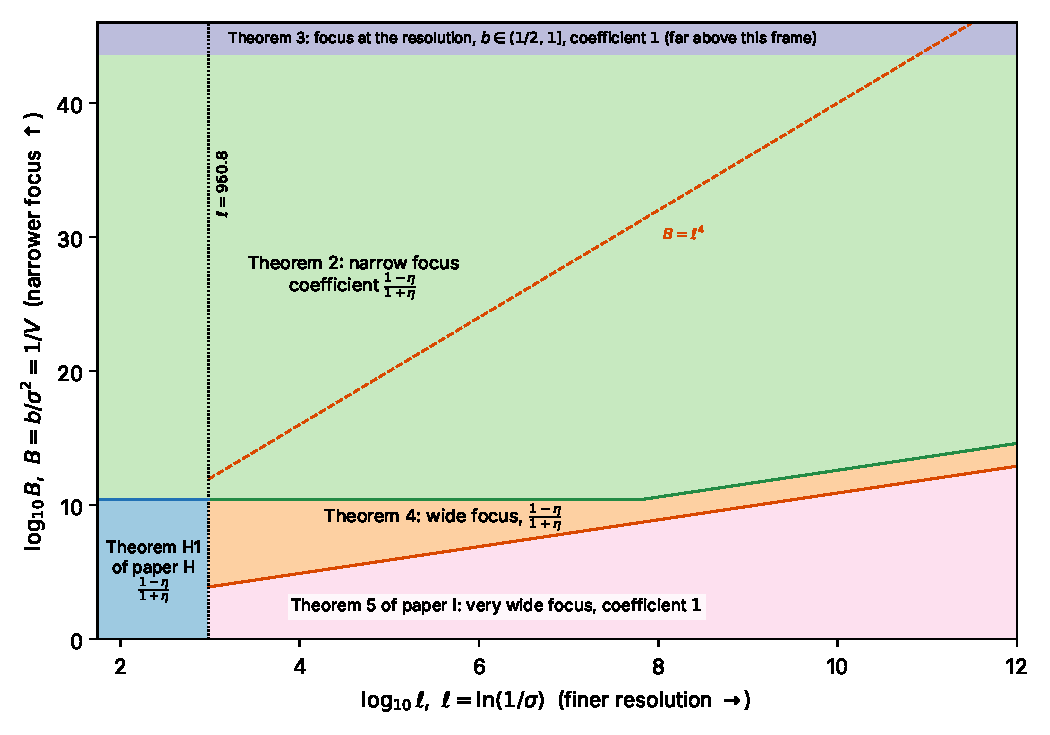
\includegraphics[width=\columnwidth]{figures/fig_map_J.pdf}
\caption{The map of the states in the $(\ell,B)$ plane, $B=b/\sigma^2$, with the coefficient that each room proves for every admissible window: $(1-\eta)/(1+\eta)=\lambda/\Upsilon$ in the narrow and wide rooms and in Theorem~H1 of~\cite{H}, one at the resolution and in the very wide room. The boundaries are those of Paper~I~\cite{I}.}
\label{fig:map}
\end{figure}

\subsection{Proof of Theorem~\ref{thm:J} from the rooms}
\begin{proof}
The case split is that of Theorem~1 of~\cite{I} (Sec.~II~C there), word for word, with the four rooms of Table~\ref{tab:rooms} in place of those of~\cite{I}.
Each room gives $(a)+(a')\ge c\,\Gamma_\ell$ with $c\in\{1,\lambda/\Upsilon\}$, so $c\ge\lambda/\Upsilon$; Theorem~H1 gives the bound on $g\sqrt\ell$ directly, with $1+12.1/\ell+2.5\times10^{-4}\ge1$.
Eq.~\eqref{eq:ga} and $\Gamma_\ell\sqrt\ell=\sqrt{1+10/\ell}$ give both statements.
\end{proof}

\subsection{What is borrowed and what is new}
\begin{itemize}
\item Borrowed unchanged: Eq.~\eqref{eq:ga} and the class conditions~\cite{F}; Theorem~H1, Lemma~CM-1, Lemma~R$_\theta$ and the sandwich~\cite{H}; the local lemmas, the 37 lines with $\eta$ as a parameter, the brightness lemma (H$'$), Lemma~$G=0$, the rule of the proof and Theorem~5~\cite{I}.
\item New here: the chord lemma (Lemma~\ref{lem:chord}) and the scaled target (Sec.~\ref{sec:sandwich}); the repaired step of FrB1 (Sec.~\ref{sec:changes}); the constants of the rule, the 18 new quoted bounds, the allocation of the remainder budget and the tail (Sec.~\ref{sec:changes}, Apps.~\ref{app:B}--\ref{app:C}); the interval proofs at the two ends (App.~\ref{app:D}); the hand proof of Theorem~\ref{thm:Jres} for every ripple (Sec.~\ref{sec:res}).
\end{itemize}

\section{The sandwich, the two ends, and the chord}
\label{sec:sandwich}

\subsection{The target scaled by the sandwich ratio}
In Paper~I the target of the narrow and wide rooms is $\Gamma_\ell\sigma\,\mathrm{den}$, and the 37 lines of App.~B of~\cite{I} are lower bounds of $\mathrm{Num}-\gamma\sigma\,\mathrm{den}$ with $\gamma=\Gamma_\ell$, written for a general $\eta\le\tfrac14$ and evaluated at $\eta=1/\ell$.
Here the target is $(\lambda/\Upsilon)\Gamma_\ell\sigma\,\mathrm{den}$.
The lines split into three kinds:
\begin{itemize}
\item \emph{gains of the sandwich} (P2z, hFz, cKz): they carry $\mathrm{fl}=1/(1+\eta)=\lambda$;
\item \emph{the target} (d1--d4): d2 and d4 come from the part $S_2$ of the denominator and carry $1/(1-\eta)=\Upsilon$; d1 and d3 come from the background part and do not;
\item \emph{remainders} (the other 28 lines, and the remainder parts of P2z, d1 and d3): functions of $\eta$ that vanish or stay bounded as $\eta\to0$.
\end{itemize}
Multiplying the target by $\lambda/\Upsilon$ turns d2 and d4 into $\lambda\gamma G/2$ and $\lambda\gamma G_\mu/(2(2+r)4r)$: the factor $\Upsilon$ cancels.
d1 and d3 are multiplied by $\lambda/\Upsilon=2\lambda-1$, Eq.~\eqref{eq:sandwich}.

\emph{This is special to the ripple sandwich.}
Paper~H's scaling step (\Hsec{IV}) uses only $\Upsilon\ge1$ for the background part, $(\lambda/\Upsilon)d_{\rm bg}\le\lambda d_{\rm bg}$, so that it holds for any pair of sandwich factors (also those of Lemmas S and S$'$).
That weaker form does not close the proof here: at $\eta=\tfrac14$, $\ell=55.26$ it lowers the margin of Case~I (option Fz) from $+0.0034$ to about $-0.019$ (App.~\ref{app:D}).
We use the identity $\lambda/\Upsilon=2\lambda-1$, which holds because $\lambda$ and $\Upsilon$ come from the same $\eta$.
The theorem is therefore stated for the ripple sandwich only.

\subsection{The chord}
After the scaling, every line is a function of $\lambda$ and of $\eta$.
For a window, $\eta=1/\lambda-1$.
The next lemma makes every line affine in $\lambda$, so that the proof at the two ends covers every ripple.

\begin{lemma}[the chord] \proofst
\label{lem:chord}
Let $f_1,\dots,f_m$ be non-negative, non-decreasing and convex on $[0,\tfrac14]$, and let $R$ be a sum of products of the $f_i$ with non-negative coefficients.
Then $R(\eta(\lambda))$, $\eta(\lambda)=1/\lambda-1$, is convex in $\lambda$ on $[\tfrac45,1]$, and
\begin{equation}
R(\eta(\lambda))\le R(0)+\bigl(R(\tfrac14)-R(0)\bigr)\,5(1-\lambda)
\label{eq:chord}
\end{equation}
for $\tfrac45\le\lambda\le1$.
The six functions
\begin{gather}
\eta,\quad \eta^2,\quad \frac1{1-\eta},\quad \frac1{(1-\eta)^2},\\ \sqrt{\mathrm{CZ}}=\frac{\eta}{\sqrt e\,(1-\eta)},\quad \frac{1+\eta}{1-\eta},
\end{gather}
and the affine $1+\eta$, are of this kind.
\end{lemma}

\begin{proof}
For two such functions, $(fg)'=f'g+fg'\ge0$ and $(fg)''=f''g+2f'g'+fg''\ge0$; induction gives products, and sums are immediate.
$\eta(\lambda)$ is decreasing and convex: $\eta'=-1/\lambda^2$, $\eta''=2/\lambda^3$.
So $(R\circ\eta)''=R''(\eta)\eta'^2+R'(\eta)\eta''\ge0$.
A convex function lies under its chord; $\eta(1)=0$ and $\eta(\tfrac45)=\tfrac14$.
For the six functions, each derivative up to the second is a non-negative rational function of $\eta$ on $[0,\tfrac14]$.
\end{proof}

\emph{The remainders are of this kind.}
App.~\ref{app:A} lists, for each of the 37 lines, the basic functions it contains (Table~\ref{tab:inventory}).
The list was read from the code of the lines by a parser that types every sub-expression: $\eta$-free and non-negative; non-negative, non-decreasing and convex (sums and products of such, division by $\eta$-free positive quantities and by powers of $1-\eta$, and the square root of CZ only); the sandwich factor $\mathrm{fl}$; and $\mathrm{ringf}=1-q$.
Every loss and target line is in the convex class; every gain is $\eta$-free, or $\mathrm{fl}$ times an $\eta$-free quantity, or $\mathrm{ringf}\cdot\mathrm{fl}$ times one \status{computer-assisted: App.~\ref{app:A}}.
Three wrong versions, a loss line multiplied by $1-\eta$, a factor $1+\eta$ replaced by $1/(1+\eta)$, and $\sqrt\eta$ in a line, are rejected by the parser.

\emph{Where a remainder multiplies the sandwich.}
Three places mix the two; they are split first, with $\lambda\le1$ and $2\lambda-1\le1$:
\begin{gather}
\lambda\,(1-q)\ \ge\ \lambda-q \qquad(\text{P2z and }\theta_0,\ q\ge0),\\
(2\lambda-1)\,k_1(\eta)\ \le\ (2\lambda-1)(1+0.184k_E)+\eta k_E\qquad(\text{d1}),\\
(2\lambda-1)(1+2\eta k_E)\ \le\ (2\lambda-1)+2\eta k_E\qquad(\text{d3}),
\end{gather}
with $k_1(\eta)=1+(\eta+0.184)k_E$.
After the split, each line is $c_0+c_1\lambda+R(\eta)$ with $\eta$-free $c_0,c_1$ and a remainder $R$ of Lemma~\ref{lem:chord} (with a sign), and Eq.~\eqref{eq:chord} replaces it by an affine function of $\lambda$.

\subsection{The two ends}
Write $\Lambda_k(a;\lambda)$ for the sum of the lines of option $k$ after these replacements.
It is affine in $\lambda$ and is a lower bound of $\mathrm{Num}-(\lambda/\Upsilon)\gamma\sigma\,\mathrm{den}$ for every window with $\eta=1/\lambda-1$.
At $\lambda=1$ it is the sum of the lines with $\eta=0$ in every remainder; at $\lambda=\tfrac45$ it is the sum with $\eta=\tfrac14$, gains at $\tfrac45$ and target $\tfrac35\gamma$ on d1, d3 and $\tfrac45\gamma$ on d2, d4.
We call these the ends A and B.

\emph{The rule does not depend on $\lambda$.}
The proof of Paper~I chooses, for each state and each $a$, one option $k$ by a rule (\Isec{IV~A}): Case~I if $G\le c_1\sqrt b/\Gamma_2$, Case~II otherwise, with thresholds $c_T$, $c_{\rm ch}$ and $a_s=4c_m^2\ell^6\sigma^3/r$.
In this paper the rule uses fixed numbers:
\begin{gather}
c_1=0.77,\qquad c_T=6.5,\qquad \Gamma_2:=\Gamma_\ell/2,\\
c_{\rm ch}=1.5\ \ (\ell<960.8),\qquad c_{\rm ch}=2.0\ \ (\ell\ge960.8),
\end{gather}
and $c_m$ at its largest value over the range, $c_m=2X_{1,B1}(\tfrac14)\sqrt{2+r}/(\tfrac34\cdot\tfrac45(1-z_2/2)\sqrt{2\pi})$.
The rule may depend on $\ell$ and on the state, but not on $\lambda$; so the option chosen at a state does not depend on $\lambda$.
Since the target part of d2 is $\lambda\Gamma_\ell G/2\le\Gamma_2G$, the inequality that defines Case~I bounds the target for every $\lambda$; inside Case~I the option Fz needs $c_{1F}-K_F/\sqrt b-\lambda c_1\ge0$ (App.~\ref{app:D}).

\begin{proposition}[two ends suffice] \proofst
\label{prop:ends}
If, for every state of a room and every $a$, the option $k$ chosen by the rule has $\Lambda_k(a;1)\ge0$ and $\Lambda_k(a;\tfrac45)\ge0$, then $\Lambda_k(a;\lambda)\ge0$ for every $\lambda\in[\tfrac45,1]$, and every window of the class satisfies $(a)+(a')\ge(\lambda/\Upsilon)\Gamma_\ell$ in that room.
\end{proposition}

\begin{proof}
$\Lambda_k(a;\cdot)$ is affine and $k$ does not depend on $\lambda$.
For a window with ripple $\eta\le\tfrac14$, $\lambda=1/(1+\eta)\in[\tfrac45,1]$, and $\Lambda_k(a;\lambda)\le\mathrm{Num}-(\lambda/\Upsilon)\Gamma_\ell\sigma\,\mathrm{den}$ at that $a$; $\Lambda_k(a;\lambda)\ge0$ for every $a$ in the range of the room gives the bound as in~\cite{I}.
\end{proof}

The interval proofs of App.~\ref{app:D} check the hypothesis of Proposition~\ref{prop:ends} at the two ends.
Each end is the proof of Paper~I with other numbers: the case analysis inside the proof ((m1)--(m4), (b.1)--(b.6)) may differ between the ends, since only the rule must be common.

\emph{In the observer's words.}
As far as each entry of the bookkeeping is concerned, a ripple of any strength between zero and $\tfrac14$ behaves like a mixture of the two extremes, no ripple and the strongest one.
Its true cost is never above that mixture, because the costs bend upwards; so checking the two extremes with one and the same rule of focus is enough for every ripple in between.

\section{What changes against Paper~I}
\label{sec:changes}

Paper~I's proofs of the narrow and wide rooms (Secs.~IV and~VI of~\cite{I}) are used here step by step.
We read every lemma behind them again, those of~\cite{I} and those it borrows from~\cite{F,H}, for the way it uses $\eta$; the result is Table~\ref{tab:lemmas} (App.~\ref{app:lemmas}) \proofst.
Every lemma uses $\eta$ only through $\eta=\sup|R|$ and $h\ge1-\eta$, that is, through $\eta<1$, or not at all; its statement carries the class bound $\eta\le1/\ell$ only through the evaluation $\eta=1/\ell$ of the coefficients of the lines.
Exactly one written step needs $\eta\le1/\ell$ as an inequality, the first step of the group FrB1 (App.~B of~\cite{I}); it is repaired below.
Besides the lemmas, the proofs of the rooms use $\eta\le1/\ell$ only through numbers: values quoted at $\eta=1/\ell$, and the tail $[10^6,\infty)$, where $(1-\eta)/(1+\eta)\ge1-2/\ell$ was used.
Both are replaced by new constants below; no step needs a new idea.
The reading was also checked numerically, by evaluating at $\eta=\tfrac14$ every lemma piece against its line on the states of the audit of~\cite{I}, and every elementary step of the 30 groups of formulas (App.~B of~\cite{I}) \numst: only the step below breaks (Sec.~\ref{sec:break}).

\subsection{The step of FrB1}
In the group FrB1 (the lines B1m, B1c, B1l, uB2c, uB2s), App.~B of~\cite{I} bounds $\hat c_0=U_1/(\sqrt2(1-\eta))+\sqrt{\mathrm{CZ}/2}\sqrt A$ by $X_1/\sqrt2$, $X_1=\tfrac43U_1$, using $U_1(\tfrac43-1/(1-\eta))\ge\sqrt{\mathrm{CZ}}$.
For $\eta=1/\ell$ the left side is at least $0.83$; for $\eta=\tfrac14$ it is zero, and the step fails (at $\ell=55.26$ on $1676$ of $1726$ audit points).
The repair is a larger factor in the one line B1m, a function of $\eta$:
\begin{equation}
X_{1,\rm B1}(\eta)=\frac{U_1}{1-\eta}+\sqrt{\mathrm{CZ}(\eta)}
\end{equation}
(at the end A, $\eta=0$: $X_{1,\rm B1}=U_1$; at the end B, $\eta=\tfrac14$: $X_{1,\rm B1}=\tfrac43U_1+\sqrt{\mathrm{CZ}(\tfrac14)}$).
Then $\hat c_0\le X_{1,\rm B1}(\eta)/\sqrt2$ holds at every $\eta$, from $A\le1$ alone.
$X_{1,\rm B1}$ is a sum of two basic functions of Lemma~\ref{lem:chord}, $1/(1-\eta)$ and $\sqrt{\mathrm{CZ}}$, so the line B1m stays in the class of that lemma; the parser reads B1m with $X_{1,\rm B1}(\eta)$ in it (Table~\ref{tab:inventory}, \code{ea\_convex.py}), and the interval proofs evaluate it at each end.
The constant $c_m$ of the rule, which must not depend on $\lambda$, takes its largest value, at $\eta=\tfrac14$ (Sec.~\ref{sec:sandwich}).
The other step of the chain, $\hat c_0^2\le X_1^2+\mathrm{CZ}$, follows from $(p+q)^2\le2p^2+2q^2$ and $1/(1-\eta)\le\tfrac43$, also at $\eta=\tfrac14$; so B1c and the other lines of the group are unchanged.
At $\ell=55.26$ and the end B the factor $X_{1,\rm B1}/X_1$ is $1.057$, inside the slack of the group (smallest ratio $1.29$ in~\cite{I}).
No new lemma is needed.

\subsection{The rule and the proof constants}
The rule constants are $c_1=0.77$, $c_T=6.5$, $c_{\rm ch}=1.5$ for $\ell<960.8$ and $2.0$ for $\ell\ge960.8$ (Paper~I: $0.78$, $3.5$, $2.9$), with $\Gamma_2=\Gamma_\ell/2$ and $c_m$ fixed (Sec.~\ref{sec:sandwich}).
They were chosen on a grid ($c_1\in[0.60,0.79]$, $c_{\rm ch}\in[1.2,2.4]$, $c_T\in\{5,6.5,8\}$) for the largest smallest margin over the two ends at $\ell=55.26$ and $960.8$ \numst.
The binding pair is the end A, where Case~I (option Fz) needs $c_1\le c_{1F}-K_F\approx0.80$, against the end B, where the chirp step (II-ch) and the rest step (II-s) need $c_1$ large.
The wide room ($\ell\ge960.8$, $B\ge8\ell+100$) has a looser bound on the chirp, $z_2\le\tfrac12$ instead of $0.01$, and at the end B it needs $c_{\rm ch}\approx2$ to balance (II-ch) against (II-s); since the rule may depend on $\ell$ but not on $\lambda$, we take $c_{\rm ch}=2.0$ for every $\ell\ge960.8$, in both rooms.
With the remainders at $\bar\eta$ at both ends (instead of the chord) the end A would need $c_1\le0.575$, and no rule closes at $\ell=55.26$ (best margin $-0.025$) \numst; the chord removes this conflict.

Inside the proof, three numbers depend on the end:
\begin{itemize}
\item the coefficient of $A2k/cKz\le A_{2C}\,b^2$ in Case~II ((R7), (m3), (m4)): $A_{2C}=2.1$ at A and $3.5$ at B, from $2/((1-\eta)\lambda k_f)$ (the wide room, with $k_f\ge0.958$, needs $3.479$ at B);
\item the allocation of the remainder budget $\mathrm{es}=10^{-11}$: (R1) $\le0.9\,\mathrm{es}\,$P1 and (R3) $\le0.1\,\mathrm{es}$ (Paper~I: $0.52$ and $0.48$). At the end B, $\mathrm{N2}/\mathrm{P1}=Q_2/(8B)$ alone is $0.601\,\mathrm{es}$, while (R3) needs $0.04\,\mathrm{es}$. The total charged to P1 is still at most es, so (R4), $e_0$, $m_1$, $m_4$ and everything after are as in~\cite{I};
\item $e_0=2\times10^{-5}$ in place of $1.26\times10^{-5}$: the absorption (R4) of the constant lines needs $e_0\ge1.637\times10^{-5}$ at the end B. $e_0$ enters $m_1=1-\varepsilon_1-e_0$ and $m_4=1-\varepsilon_h-e_0$; the condition ``$e_0$ needed $\le e_0$'' is checked on every piece, and every later step uses $m_1$, $m_4$ only through the interval values. The lower end of $b$ (the bound $b_0$ and $K_F$ of (R5)) does not involve $e_0$. In the wide room, where $B\ge B_m=8\ell_a+100$ on a piece, $e_0=2.7/\sqrt{B_m}+\mathrm{es}$ (Paper~I: $2/\sqrt{B_m}+\mathrm{es}$); there $e_0$ needed is at most $0.967\,e_0$.
\end{itemize}

\subsection{The quoted bounds}
The proof of~\cite{I} quotes $48$ numbers as valid for every $\ell$ (App.~C there).
At both ends $30$ of them still hold; $18$ take new values, each the largest (or smallest) interval value over the two ends, all pieces and the tail, rounded outward to four digits.
They are listed in Table~\ref{tab:quoted} (App.~\ref{app:B}) and checked on every piece by the second run of App.~\ref{app:D}.
The largest changes come from the remainders at $\eta=\tfrac14$: $\varepsilon_1\le0.2013$ (was $0.01457$), $\varepsilon_h\le0.3882$ (was $0.1808$), $\theta_{\rm bg}\ge0.699$ (was $0.8985$), $c_{1F}\ge0.6203$ (was $0.7857$).

\subsection{The tail}
On $[10^6,\infty)$ Paper~I replaced two exact quantities by tail-safe bounds that used $\eta=1/\ell$: the line $A=(1-\eta)/((1+\eta)\Gamma_\ell\sqrt\ell)\ge1-7/\ell$.
With $\eta$ and $1/\ell$ separated, $A\ge1-a_1/\ell$ with $a_1=5+\ell(1-\theta_A)$, where $\theta_A$ is the ratio of gain to target in $A$ (App.~\ref{app:C}).
In Paper~I $\theta_A=(1-\eta)/(1+\eta)$ with $\eta=1/\ell$, so $a_1=7$; here the ratio is one and $a_1=5$.
With $a_1=7$ the general formulas reproduce the tail of~\cite{I} exactly (every one of the $101$ interval values on $[10^6,\infty)$ is the same).

\section{Focus at the resolution: the coefficient stays one}
\label{sec:res}

\begin{proposition}[line form] \proofst
\label{prop:Jres}
Let $\ell\ge55.26$ and let the ripple satisfy $\eta\le\bar\eta=\tfrac14$.
Let a state satisfy $\tfrac12<b\le1$, $\mu>0$, $\sigma^3\le r\le\tfrac14$, $\kappa>0$, and let $P>0$ satisfy (A), (K), (CM) of the brightness lemma of~\cite{I}.
Then for every $a>0$ and every $\gamma\in[0,0.49]$ the lines of the option Fz satisfy $\Lambda_{\rm Fz}(a)\ge0$, with the target $\gamma\sigma\,\mathrm{den}$ (coefficient one).
\end{proposition}

\begin{proof}[Proof of Theorem~\ref{thm:Jres}]
If $G>0$, the lines of option Fz (valid for $b\in(\tfrac12,1]$, Sec.~V of~\cite{I}) and Proposition~\ref{prop:Jres} with $\gamma=0.49$ give $(a)+(a')\ge0.49$.
If $G=0$, Lemma~$G=0$ of~\cite{I} gives $(a)+(a')\ge0.1995$; it concerns a window without a ripple in the focus and uses no bound on $\eta$.
Both exceed $\Gamma_\ell\le0.1462$.
\end{proof}

\emph{Why the coefficient stays one.}
Option Fz uses only the two background lines P1, P4z and the ripple-free part of P3z; the gain P2z enters only to absorb $\mathrm{d4}+\mathrm{N4G}$.
No gain carries the sandwich factor $\lambda$, so nothing has to be scaled; the ripple enters only through the remainders, which we bound uniformly at $\bar\eta=\tfrac14$, and through $k_2=1/(2(1-\eta))\le\tfrac23$ in the target.

\subsection{Proof of Proposition~\ref{prop:Jres}}
The steps are those of Sec.~V of~\cite{I}, with $\eta=\tfrac14$ in every remainder.
Every term below is a product of non-negative factors that do not increase with $\ell$ ($1/\ell$, $\sigma$, $\ell\sigma$, $\sqrt\sigma$, $U_1^2/\ell$, $X_1^2/\ell$; $\eta=\tfrac14$ is fixed), so $\ell=55.26$ is the worst case.
Every number is an exact rational upper or lower bound: $e\ge2.71828$, $e^{-x}\le2.71828^{-\lfloor x\rfloor}/\sum_{j\le3}f^j/j!$ ($f=x-\lfloor x\rfloor$), $\sqrt{0.2}\le0.44722$, $\sqrt\pi\ge1.7724$, $\sqrt2\ge1.4142$, $P_1\le0.8829$ ((F1$'$) of~\cite{I}, which does not involve $\eta$); each square root is checked by squaring.
\begin{itemize}
\item[(R1$'$)] N1 $=\varepsilon_1(r)$P1 with $\varepsilon_1\le\bar\eta k_E\cdot1.8\le0.2013$; the other L-lines are at most $e_L$P1, $e_L\le2.06\times10^{-14}$ (the largest terms are A2b and B2b, of order $\sqrt\sigma\,\bar\eta^2$); $\mathrm{d4}+\mathrm{N4G}\le1.4\times10^{-4}\,\mathrm{es}_\sigma\,$P2z.
\item[(R2$'$)] hneg1 $=\varepsilon_h(r)$P4z, $\varepsilon_h\le2k_E(\bar\eta+0.184)/\omega\le0.3882$.
\item[(R3$'$)] The S-lines are at most $e_S$P4z ($a\le1$) or $e_S$P1 ($a\ge1$), $e_S\le4.0\times10^{-13}$ ($c_S\le0.1985$). So $e_L+e_S\le e_2=10^{-12}$, with room $5.8\times10^{-13}$.
\item[(R4$'$)] $\mathrm{N3}+\mathrm{M0Xi}+\mathrm{A1v}+\mathrm{pair}\le1.9165\,\sigma\le2\sigma$. (Paper~I had $1.86\sigma$; at $\bar\eta=\tfrac14$ this bound fails, and $2\sigma$ is still covered by the tail term below for $\ell\ge1.5$.)
\item[(R5$'$)] $\mathrm{FzK}+\mathrm{A2k}+\mathrm{B2a}\le0.0682\,\ell\sigma\le\ell\sigma$.
\end{itemize}
The chain $\varepsilon_1$, $\varepsilon_h$, $\theta^2$, $k_1$ and the two margins below are checked step by step in exact rationals, each from the printed bounds before it (\code{dy\_room2\_hand.py}).
Hence, as in~\cite{I}, for every $a>0$,
\begin{equation}
\Lambda_{\rm Fz}(a)\ \ge\ \theta\sqrt b-\gamma k_1b-\gamma k_2G-(2\ell+\tfrac12)\sigma,
\end{equation}
with $\theta^2\ge(1-\varepsilon_1-e_2)(1-\varepsilon_h-e_2)\omega\ge0.48864$, $k_1=1+(\bar\eta+0.184)k_E\le1.19413$, $k_2=\tfrac23$ and $G\le P_1/3$.
The right side is concave in $b$; at the ends, in squared form with $\gamma=0.49$,
\begin{gather}
b=1:\quad \theta^2-\bigl(\gamma k_1+\gamma k_2P_1/3+\text{tail}\bigr)^2\ \ge\ 0.0245,\\
b=\tfrac12:\quad \theta^2-2\bigl(\gamma k_1/2+\gamma k_2P_1/3+\text{tail}\bigr)^2\ \ge\ 0.186 .
\end{gather}
$\Lambda_{\rm Fz}$ decreases in $\gamma$, so the bound holds on $[0,0.49]$.
Case~I of the rule holds throughout: $c_1\sqrt{1/2}/\Gamma_2-P_1/3\ge7.15$ with $c_1=0.77$, $\Gamma_2=\Gamma_\ell/2$.
\qed

\emph{What is hand and what is computed.}
Every inequality above is closed by hand: the arithmetic of the rational bounds is done exactly (by \code{fractions}), and nothing is evaluated in floating point or interval arithmetic.
The same quantities were also enclosed by interval arithmetic on $[55.26,\infty)$ as one piece, and the hand bounds lie above the interval values.
At $\gamma=\Gamma_{55.26}\le0.1462$ the margin at $b=1$ is $0.496$, so the law with coefficient one has room to spare.
The proof gives $0.49$ in place of the $0.6$ of~\cite{I} for a weak ripple; for $\eta\le1/\ell$ the $0.6$ of~\cite{I} stands.
With $\gamma=0.51$, or with $\bar\eta=0.3$, the bound at $b=1$ is negative.

\emph{In the observer's words.}
A focus as narrow as the resolution sees less than a hundredth of a period.
The ripple can only darken what it sees.
Even the strongest ripple of the class leaves the two background terms: wherever the ripple reaches the focus ($G>0$) they keep $(a)+(a')$ at $0.49$ or more, more than three times the $\Gamma_\ell\le0.146$ that the law asks for; where it does not, $(a)+(a')\ge0.1995$, still above it.

\section{Trying to break it}
\label{sec:break}

Before the interval proofs we tried to break the claim and the lines it rests on.
For every search we report the families, planted adversaries, and deliberately wrong versions that the same search does break.
Everything in this section is \numst.

\subsection{The lines against the lemmas at a strong ripple}
The audit of~\cite{I} (Sec.~VIII and App.~B there) compares every lemma piece with its line on families of states: uniform, edges, corners, several edges at once, large $b$, with the brightness at its ceiling for the corner family, and a grid of $a$ with its end points.
We ran it with the lemma at the ripple $\eta\in\{1/\ell,0.05,0.15,0.25\}$, the target $\gamma(1-\eta)/(1+\eta)$, and the lines of this paper at $\lambda=1/(1+\eta)$, in both forms (remainders at $\bar\eta$, and the chord), for $\ell\in\{55.26,960.8,10^4,10^6,10^{12}\}$: $94\,512$ points, no group and no option total violated (tolerance $10^{-30}$ relative).
Wrong versions, each at $\eta=\tfrac14$ and $\ell\in\{55.26,960.8\}$: the remainders at $1/\ell$ (``$\eta$ forgotten''), $5\,554$--$7\,200$ violations; the target not scaled, $1\,886$--$2\,137$; P2z$\times1.01$, $485$--$646$; N1$\times0.99$, $511$--$687$; B2c$\times0.99$, $470$--$474$; the five lines of FrB1$\times0.70$, $416$--$441$.
The old constant $X_1$ in B1m is \emph{not} seen by this audit, because the group FrB1 has slack; it breaks the written step of the chain, which the next audit checks.

The 30 groups of formulas of~\cite{I} (lemma piece, closed form, elementary steps, line) were evaluated at $\eta=\tfrac14$ for $\ell\in\{55.26,955.8,10^6,10^{12}\}$.
With the steps of~\cite{I}, only FrB1 breaks, in its first step; with $X_{1,\rm B1}$ no group breaks.
Wrong versions: the new line with the old step ($449$ and $229$ failing points), and the new step at $\eta=0.3>\tfrac14$ (FrB1 and FrB2 break).

At $\eta=1/\ell$ the published audits of~\cite{I} are reproduced exactly by the code of this paper, in which $\eta$ and $1/\ell$ are separate arguments (App.~\ref{app:E}).

\subsection{The conclusion}
We searched for states where the lines of this paper give $(F^2-1)\ell<10$, with $F=\min_a\max_k$ of the ratio of the best option to the target (the quantity of Sec.~VIII of~\cite{I}), at the ends A and B in both forms and, for the form with the remainders at $\bar\eta$, at $\lambda=0.9$.
The families are the twelve of~\cite{I} (corner, global, five edge families, five narrow families) and the minimisers of the searches of~\cite{I} as seeds; $n=800$ walkers per family, shrinking random walks and pattern search.
\begin{center}
\small
\begin{tabular}{lccccc}
$\ell$ & A & mid & B & A (chord) & B (chord)\\ \hline
$55.26$ & $22.89$ & $23.66$ & $24.54$ & $22.89$ & $24.54$\\
$960.8$ & $28.22$ & $28.66$ & $29.16$ & $28.22$ & $29.16$\\
$10^4$ & $35.83$ & $36.25$ & $36.73$ & $35.83$ & $36.73$\\
$10^6$ & $51.83$ & $52.26$ & $52.73$ & $51.83$ & $52.73$\\
\end{tabular}
\end{center}
The smallest value, $22.89$, is more than twice what the claim needs.
The forms agree at the minimisers because there $k_E\approx\sqrt r$ is small and the remainders hardly act; the minimum moves from Paper~I's $17.56$ to $22.89$ because the end A has gains at factor one instead of $1/(1+1/\ell)$.
Before the interval proofs, the corner family at $\ell=55.26$ was searched once more with $n=1500$ at both ends: $22.89$ and $24.54$.

Power: dropping a main gain line (P2z, or hFz) makes the margin negative at both ends and both $\ell$ (8 versions); the three planted dips of~\cite{I} (corner, narrow, low $\mu$; depth 5) were found, $11$ of $12$ at once and the last one (corner, end A, $\ell=55.26$) with $n=1500$ or with the widths tripled; the corner dip was found again by the $n=1500$ search at both ends.
A first design of the planted dip (width $0.5$ next to the minimiser) was too narrow to be felt by the walkers at $\ell=55.26$; we replaced it by the design of~\cite{I} and report it here.

\emph{In the lines of this proof, the coefficient cannot be one.}
With the target not scaled ($\gamma$ in place of $(\lambda/\Upsilon)\gamma$) at $\eta=\tfrac14$, the smallest $(F^2-1)\ell$ of the lines is $-26.5$ at $\ell=55.26$ and $-604$ at $\ell=960.8$: $F$ falls to about $3/5$, the sandwich ratio.
This is a statement about the lower bounds of this proof, not about $g$.
The sandwich puts the worst gain factor $\lambda$ and the worst cost factor $\Upsilon$ at the same time; in one window the two need not occur together.
The next subsection asks what the true quantity does.

\subsection{The true quantity at a strong ripple}
\label{sec:truth}
We computed the true quantity $Q=(a)+(a')$, which bounds $g$ through Eq.~\eqref{eq:ga}, on windows with $\eta=\tfrac14$, $0.1$ and $1/\ell$, and searched for small $Q\sqrt\ell$ \numst.

\emph{The method.}
The quantity of \code{dp\_truth.py} of~\cite{I} is a two-dimensional quadrature in $(v,w)$ and works only for moderate $\sigma$.
We write it in the variables of the local lemmas of~\cite{I}.
The integrand is split into a sum of terms (a function of the ripple phase $t$) $\times\,\hat s^k\times\{1,\,1-\cos(\sqrt y\hat s),\,\sin(\sqrt y\hat s)\}$, $k\le2$; the nonlinearity in the ripple, $1/h$ included, stays inside the functions of $t$.
These are sampled on $M$ points and replaced by their discrete Fourier coefficients up to a cut $n_{\rm cut}$; the Gaussian averages $E[\hat s^kU_j(\hat s)e^{in\sqrt\tau\hat s}]$ are then taken in closed form.
For a narrow focus the $\hat s$-average is done instead by $128$-point Gauss--Hermite quadrature; the $w$-average by Gauss--Legendre panels at the two scales $s$ and $L$ (for $L>3$, the part without ripple in the closed form of Lemma~11 of~\cite{I}).
$1-\cos$ is written without cancellation, and everything is in extended precision, so that $\sigma=e^{-960.8}$ is representable.
No term is expanded or dropped; the only errors are those of the quadratures and of the Fourier truncation and aliasing.
Checks: against the quadrature of~\cite{I} at $\ell=8$ ($44$ comparisons, relative difference at most $1.1\times10^{-5}$, the error of that quadrature), against the closed form of Lemma~11 of~\cite{I} at $\ell=8$, $55.26$, $960.8$ ($27$ states, $2\times10^{-15}$), and the grids doubled ($5\times10^{-12}$); every value reported is computed on the finer of the two $t$-grids of the code.

\emph{The windows and states.}
Windows are built from a non-negative unblurred profile with (P2) and (P3), aligned so that $\sup|R|=\eta$ exactly: one harmonic; two harmonics ($m=3,21,61$); a spike (all harmonics up to the blur); a packet of fine harmonics at the trough of the fundamental, where $h=1-\eta$ (the shape that brings the worst cost and the worst gain of the sandwich closest together), and the same packet at the crest.
States: the narrow room (Theorem~\ref{thm:Jnarrow}), the focus at the resolution (Theorem~\ref{thm:Jres}) and the band $8\ell+100\le B<\ell^4$ of Theorem~\ref{thm:Jwide}, all states, and separately the ripple-dominated states (the ripple carries at least half of the denominator).
Search: $400$ points of the unit cube of the parameters, then Nelder--Mead from the best six, for each of the $126$ combinations at $\ell=55.26$; the minimisers re-evaluated on finer grids; the best combinations again at $\ell=200$ and $960.8$.

\emph{The result.}
\begin{center}
\small
\begin{tabular}{lccc}
smallest $Q\sqrt\ell$ found & $\eta=\tfrac14$ & $\eta=0.1$ & $\eta=1/\ell$\\ \hline
$\ell=55.26$ & $3.40$ & $3.49$ & $5.20$\\
$\ell=200$ & $10.3$ & $20.0^*$ & $8.84$\\
$\ell=960.8$ & $22.1$ & $17.1$ & $29.3$\\
\end{tabular}
\end{center}
At $\ell=200$ and $960.8$ only the best combinations of $\ell=55.26$ were searched, with a smaller budget, so these are upper estimates of the minimum (${}^*$: the search ended at a dark ripple).
The smallest values sit in the narrow room, at packets of fine harmonics whose local fineness is $\mu\approx1.2$; there $Q\approx1/(2\sqrt\mu)$, far above $\Gamma_\ell$.
At the resolution the minimum is that of a dark ripple ($7.43$ at $\ell=55.26$, the same for every $\eta$), and in the band of Theorem~\ref{thm:Jwide} every search ends at $Q\sqrt\ell=\sqrt\ell/(8\sigma\ell^4)$, about $10^{17}$ at $\ell=55.26$ and $e^{934.7}$ at $\ell=960.8$ \derivst: there $y=1/(2B)$ is not small, a ripple that carries the denominator pays $(a)+(a')\gtrsim y/(4\sigma)=1/(8\sigma B)$ through the spread of its phase over the focus (the chirp line cKz), and a dark ripple pays the background $C_0/\sqrt b$.
The minima grow roughly like $\sqrt\ell$, since in this class the local fineness $\mu$ of a bright ripple stays near one.
At $\ell=55.26$ a strong ripple gives \emph{smaller} minima than a weak one, because it can be brighter; at $\ell=200$ and $960.8$ the values are upper estimates from a smaller budget, and their order can change with it. The comparison that does not depend on the budget is at the same window shape and the same state: there $Q$ with $\eta=1/\ell$ is $1.4$ to $3.4$ times larger than with $\eta=\tfrac14$.

\emph{Does the sandwich act in the true quantity?}
At each minimiser we also computed $Q_{h1}$, the same window and state with the factors $1/h$ of the scores replaced by one: these factors are what the ripple sandwich bounds by $\lambda$ and $\Upsilon$.
At the ripple-dominated minimisers with $\eta=\tfrac14$, $Q/Q_{h1}$ lies between $0.93$ and $1.04$ (against $(1-\eta)/(1+\eta)=0.6$).
A search that minimises $Q/Q_{h1}$ itself finds $0.71$ at $\eta=\tfrac14$ and $0.87$ at $\eta=0.1$ (against $0.6$ and $0.82$), both for the packet at the trough, as designed; but there $Q\sqrt\ell$ is $257$ and $766$.
So the factors of the sandwich do act in the true quantity, up to most of their bound, but only at states where the information is plentiful; at the states where it is scarce they move $Q$ by a few per cent.

\emph{Power.}
At the overall minimiser and at the ripple-dominated one: leaving out the term (III) of the numerator lowers $Q$ by $43$--$50\,\%$ and the search finds values near zero; the scores computed with $1-ER$ in place of $h$ change $Q$ by up to $15\,\%$ over the minimisers; a planted bowl at a random point, with its bottom at $0.3$ times the minimum, is found by the same search (bottom $1.05$, found $1.06$; and $1.02$, found $1.03$); and an artificial worst sandwich (the brightness in the denominator times $1/(1-\eta)^2$, in the numerator times $1/(1+\eta)^2$) gives $2.11$ and $2.20$ against the true $6.68$ and $3.40$ of the same family: within these families, the search would have found a lowering by the sandwich ratio; it found none.

\emph{What this shows and what it does not.}
No window found has $((a)+(a'))\sqrt\ell$ near one, let alone near $(1-\eta)/(1+\eta)$ (and $g\sqrt\ell\ge(1-\bar\varepsilon)((a)+(a'))\sqrt\ell$).
But in the regime of the class ($x\le0.003$, the fundamental the largest harmonic) the true quantity is far above $\Gamma_\ell$ for weak ripples too.
The states where the law is nearly tight are those of the comb of~\cite{F}, whose period is at the scale of the blur ($x\approx\ell/4$ for its own fundamental); there $(a)+(a')$ is $1.24/\sqrt\ell$ at $\ell=55.26$ and tends to $1/\sqrt\ell$ (\code{dh\_true.py} in the repository of~\cite{I}), and they are outside the class of Theorem~\ref{thm:J}.
So the searches do not test the factor near tightness; they show that, where they look, a strong ripple does not take a fraction of the information away.
\begin{conjecture}[coefficient one for every ripple] \conjst
\label{conj:one}
For every admissible window ($\eta\le\tfrac14$), every state and every $\ell\ge55.26$, $g\sqrt\ell\ge1-\bar\varepsilon$.
\end{conjecture}

\subsection{The convexity inventory}
The parser of Lemma~\ref{lem:chord} was itself tested with three wrong versions of the lines (a loss multiplied by $1-\eta$, $1+\eta$ replaced by $1/(1+\eta)$, $\sqrt\eta$ in d3): all three are rejected.
Our first hand-written inventory had three wrong rows (N4G, B2s, uB2s listed basic functions they do not contain); the parser found them, and Table~\ref{tab:inventory} is the corrected one.
Numerically, every product of up to three of the six functions, and every loss line of~\cite{I} at random states, lies under its chord on a grid of $\lambda$ (smallest difference $\ge-10^{-15}$ relative, rounding).

\section{Limits}
\label{sec:limits}

\begin{itemize}
\item \emph{The ripple sandwich only.}
  The coefficient $\lambda/\Upsilon=(1-\eta)/(1+\eta)$ is that of the $\eta$ sandwich.
  Paper~H also has the sharper factors of Lemmas S and S$'$, for windows whose ripple is strong but carries little energy.
  For those factors $\lambda$ and $\Upsilon$ are not tied by $\lambda/\Upsilon=2\lambda-1$, and with the general form $(\lambda/\Upsilon)d_{\rm bg}\le\lambda d_{\rm bg}$ the end B does not close (Sec.~\ref{sec:sandwich}).
  So Theorem~\ref{thm:J} gives the coefficient $(1-\eta)/(1+\eta)$ and nothing better, even for windows where Lemma S would give more.
\item \emph{The factor itself.}
  For a weak ripple the factor $(1-\eta)/(1+\eta)$ is close to one, and for $\eta\le1/\ell$ Paper~I's coefficient one is the better statement.
  For a strong ripple, the lower bounds of this proof need some factor below one (Sec.~\ref{sec:break}); the true quantity, on the windows we computed, does not (Sec.~\ref{sec:truth}) \numst.
  Whether the coefficient one holds for every ripple of the class is Conjecture~\ref{conj:one}; a proof would need a sandwich that does not put the worst gain and the worst cost together.
\item \emph{The constant $\bar\varepsilon$.} Every bound carries $1-\bar\varepsilon$ of condition (P6) of~\cite{F}; it is a hypothesis on the class.
\item \emph{The regime.} $5\times10^{11}\sigma^2\le x\le0.003$, as in~\cite{H,I}.
\item \emph{The lower side only.} The upper side of the law is that of~\cite{F}.
\item \emph{The lemmas of Paper~I at a strong ripple.} We use the lemmas of~\cite{I} with $\eta\le\tfrac14$ in place of $\eta\le1/\ell$. Table~\ref{tab:lemmas} records, lemma by lemma, where $\eta$ enters each proof and which bound it uses; one written step needed $\eta\le1/\ell$ and is repaired (Sec.~\ref{sec:changes}), and the proofs of the rooms used $\eta=1/\ell$ only in numbers, which are retaken. The reading is ours; a reader who wants to check it independently should start with Table~\ref{tab:lemmas} and App.~B of~\cite{I}.
\item \emph{The true quantity.} The searches of Sec.~\ref{sec:truth} cover the families and states listed there, at $\ell=55.26$, $200$ and $960.8$; they do not reach the nearly tight states of the law, which lie outside the class.
\item \emph{General states.} Conjecture~18 of~\cite{F}, on states outside the class of the focus coordinates used here, is not touched.
\end{itemize}


\begin{acknowledgments}
The author used AI assistants in this work. Anthropic Claude (claude-opus-5-5) extended the lemmas and the interval arithmetic to strong ripples, proved the convexity lemma, wrote the verification code, and drafted the text; a separate session re-ran and checked every stage. Google Gemini (Gemini 4 Neon) and OpenAI ChatGPT (GPT-6 Sol) independently reviewed the manuscript and re-derived its main steps; their comments led to corrected rounding in the hand proof of Theorem~\ref{thm:Jres}, a precise statement of where the bound $0.49$ applies, a consistent definition of the repaired constant of FrB1, and a more exact account of the numerical study. The author directed the research, made all decisions on its content, and takes full responsibility for this article.
\end{acknowledgments}

\emph{Data and code availability.}
All code, stored results, the interval-arithmetic computations and the verification suite are available at \url{\Jrepourl} and archived at Zenodo, doi:\Jcodedoi.
A single entry point, \code{verification/run\_all.py}, recomputes every computer-assisted part of this paper and re-derives its numbers from the stored results; \code{verification/quick.py} is a short check that runs in a few minutes.
The repository starts from the repository of Paper~I~\cite{Icode}; the certificates of Theorem~H1 are those of~\cite{H} and are re-run with the repository of~\cite{H}.
Papers~F, H and~I and their repositories are not changed.

\paragraph*{Version~1.0.}
First version.


\appendix
\section{How the lemmas use the ripple}
\label{app:lemmas}

Theorem~\ref{thm:J} uses the lemmas of Paper~I~\cite{I} and the lemmas Paper~I borrows from~\cite{F,H} with $\eta\le\tfrac14$ in place of $\eta\le1/\ell$.
Table~\ref{tab:lemmas} is the result of reading every one of their proofs again for this purpose.
For each lemma it records whether $\eta$ or $\ell$ appears in the hypotheses, the step of the proof where $\eta$ enters, the bound on $\eta$ that the step needs, whether that bound holds for $\eta\le\tfrac14$, and, where it does not, the repair.

\emph{The result of the reading} \proofst.
Every lemma uses $\eta$ only through $\eta=\sup|R|$ and $h\ge1-\eta$ (so through $\eta<1$), or not at all; the borrowed lemmas of~\cite{F} and the lemmas of Theorem~5 of~\cite{I} use the class constant $\Qb$ instead.
Theorem~H1 of~\cite{H} is stated for every admissible window, and its certificates use $\bar\eta=\tfrac12$.
Exactly one written step of the lemmas needs $\eta\le1/\ell$ as an inequality: the first step of the group FrB1, $U_1(\tfrac43-1/(1-\eta))\ge\sqrt{\mathrm{CZ}}$, whose left side is zero at $\eta=\tfrac14$ (check e3).
It is repaired by the constant $X_{1,\rm B1}$ of Sec.~\ref{sec:changes} (check e4).
Besides the lemmas, the written proofs of the narrow and wide rooms of~\cite{I} use $\eta\le1/\ell$ in two further ways, both of them numbers: values quoted at $\eta=1/\ell$ (18 of the 48 quoted bounds, and two numbers of the text, $q\le0.0026$ and $\mathrm{ringf}\ge1-0.0026$, which become $\tfrac1{240}$ and $1-\tfrac1{240}$, check e6), and the tail $[10^6,\infty)$, where $(1-\eta)/(1+\eta)\ge1-2/\ell$ was used (check e7).
Both are replaced in this paper by new constants (Table~\ref{tab:quoted}, App.~\ref{app:C}); no step needed a new idea.

\emph{What is checked by machine} (\code{dz\_lemma\_table.py}).
The rows of the table that carry lines of~\cite{I} are compared with the inventory that the parser of Lemma~\ref{lem:chord} reads from the code (Table~\ref{tab:inventory}): every basic function of $\eta$ in a line is one that the table lists for the lemma the line comes from, and every function listed for a lemma occurs in one of its lines (37 of 37 lines; three wrong versions of the table are caught).
The elementary steps (e1)--(e8) are checked at $\eta\le\tfrac14$ in exact rational or 60-digit arithmetic, each with a wrong version that fails: (e1) $|z-\ln(1+z)|\le z^2/(2(1-\eta))$ for $|z|\le\eta$; (e2) $1/(1-\eta)\le\tfrac43$; (e3) the old step of FrB1, true at $\eta=1/\ell$ and false at $\tfrac14$; (e4) the repaired step; (e5) $\hat c_0^2\le X_1^2+\mathrm{CZ}$; (e6) the ring factor; (e7) the old tail step; (e8) the factors of Theorem~H1.

% written by src/dz_lemma_table.py (stage DZ); do not edit by hand
\begin{table*}
\caption{How the lemmas behind Theorem~\ref{thm:J} use $\eta$: the re-reading of every lemma of~\cite{I} that Theorem~\ref{thm:J} uses, and of the lemmas it borrows from~\cite{F,H}. ``Statement'': $\eta$ or $\ell$ in the hypotheses. ``Where $\eta$ enters'': the step of the proof. ``Bound used'': the bound on $\eta$ that step needs. Numbers of lemmas and sections are those of~\cite{I} v1.0 unless marked H~\cite{H} or F~\cite{F}. The labels (e1)--(e8) are the elementary checks of \code{dz\_lemma\_table.py}.}
\label{tab:lemmas}
\begin{ruledtabular}
\scriptsize
\begin{tabular}{p{0.15\textwidth}p{0.09\textwidth}p{0.1\textwidth}p{0.25\textwidth}p{0.12\textwidth}p{0.08\textwidth}p{0.13\textwidth}}
lemma & where & statement & where $\eta$ enters & bound used & $\eta\le\frac14$ & repair\\ \hline
Lemma 18 (direct form) & I, App. A 2 & none & nowhere (an identity: the definition in the variables of the line) & none & yes & ---\\
Lemma 19 (M0) & I, App. A 3 & none ($|R_\theta|\le\eta$ is a consequence) & $|R_\theta|\le\eta$ from $|R|\le\eta$; $|t_\rho|\le0.184b$ uses $\Qb$ & $\eta=\sup|R|$ (definition) & yes & ---\\
Lemma 19 (A1v), (A1w) & I, App. A 3 & none & (A1w): $|R|\le\eta$ and $\eta k_E/\sqrt{\mathrm{se}_E}=\eta/L$ (identity) & definition & yes & ---\\
Lemma 19 (A2) & I, App. A 3 & none & $h\ge1-\eta$; $R^2/h\le\eta^2/(1-\eta)$ & $\eta<1$ & yes & ---\\
Lemma 19 (B1v) & I, App. A 3 & none & $\langle\hat s^2\tilde F\rangle\le\kappa W/(1-\eta)$ ($h\ge1-\eta$) & $\eta<1$ & yes & ---\\
Lemma 19 (B1w) & I, App. A 3 & none & $|G_E(R)|\le R^2/(2(1-\eta))$ for $|ER|\le\eta$; $R^2\le\eta^2$ & $\eta<1$ (checked, e1) & yes & ---\\
Lemma 19 (B2) & I, App. A 3 & none & $E|X_1|/h\le U/(1-\eta)$; $R^2/h^2\le\eta^2/(1-\eta)^2$ & $\eta<1$ & yes & ---\\
Lemmas 15, 20, 21 ($M_4$, $M_1$, $M_2$) & I, Sec. VI, App. A 3 & none & nowhere ($y$ only) & none & yes & ---\\
Lemma 22 (ring) & I, App. A 4 & none & $M=\eta^2/(1-\eta)$ for $g=R^2/h$; $q=K^2(1+\eta)/(8B(1-\eta))<1$ & $\eta<1$; $q\le\frac1{240}$ (narrow), $\frac5{24}$ (wide) at $\eta\le\frac14$ (e6) & yes & the number $1-0.0026$ in the sign paragraph of App. B of I is the value at $\eta=1/\ell$; at $\eta\le\frac14$ it is $1-\frac1{240}$ (the code computes $q$ with $\eta$)\\
Lemma 23 (pair) (a)--(c) & I, App. A 4 & none & $\tilde F$ between $E^2X_1^2/(1\pm\eta)$; tails $U^2g_s/(1-\eta)$ & $\eta<1$ & yes & ---\\
Lemma 23 (d), FrB2 & I, App. A 4; App. B (group B2c$+$B2s) & none & $c_0=\sigma U/(\sqrt2(1-\eta))+\zeta/\sqrt2$, $\zeta^2=\sigma^2\mathrm{CZ}A$; App. B: $U_1/(1-\eta)\le X_1$ & $1/(1-\eta)\le\frac43$ (e2) & yes (equality at $\frac14$) & ---\\
Lemma 23 (d), FrB1 & I, App. A 4; App. B (group B1m$+\dots+$uB2s) & none & App. B: $\hat c_0\le X_1/\sqrt2$ from $U_1(\frac43-1/(1-\eta))\ge\sqrt{\mathrm{CZ}}$; $\hat c_0^2\le X_1^2+\mathrm{CZ}$ & $\eta\le1/\ell$ in the first step (e3); $1/(1-\eta)\le\frac43$ in the second (e5) & \textbf{no} for the first step (zero left side at $\frac14$); yes for the second & $X_{1,\rm B1}(\eta)=U_1/(1-\eta)+\sqrt{\mathrm{CZ}(\eta)}$ in the line B1m (e4), a function of $\eta$ of the class of Lemma~\ref{lem:chord}, Sec.~\ref{sec:changes}\\
$v$-branch sum and its den (App. A 5 of I) & I, App. A 5 & none & den: $b(1+k_ER_\theta)\le b(1+\eta k_E)$; $W/(1-\eta)$ & $\eta<1$ & yes & ---\\
\end{tabular}
\end{ruledtabular}
\end{table*}
\begin{table*}
\addtocounter{table}{-1}
\caption{(Continued.)}
\begin{ruledtabular}
\scriptsize
\begin{tabular}{p{0.15\textwidth}p{0.09\textwidth}p{0.1\textwidth}p{0.25\textwidth}p{0.12\textwidth}p{0.08\textwidth}p{0.13\textwidth}}
lemma & where & statement & where $\eta$ enters & bound used & $\eta\le\frac14$ & repair\\ \hline
Lemma R$_\theta$ of H, $w$-branch (N1--N4, P1, P2, den) & H, Sec. IX A; \code{co\_remainders.py}; I, App. A 6 & none (``every periodic window state'') & $\Lambda_1$, $Q_2$: $|R_\theta|\le\eta$; $J_{2,\rm up}$, $M_{4w}$, $J_{\rm up}$: $\eta^2/(1-\eta)$, $D_0/(1-\eta)$; P2: $D_0/(1+\eta)$; $\xi=\sigma U_1/(1-\Qb)$ uses $\Qb$, not $\eta$ & $\eta<1$, $\Qb=\frac14$, $A\le1$ & yes & ---\\
Lemma 8 (the 37 lines): the 12 identities and 18 inequalities & I, Sec. III B; App. B & $\eta\le1/\ell$ (coefficients evaluated at $\eta=1/\ell$) & coefficients only, except the FrB1 step (row above) and $1/(1-\eta)\le\frac43$ in FrB2, FrB1; signs: positive factors for $\eta<1$ & $\eta<1$, $\eta\le\frac14$ & yes, with the FrB1 constant & the coefficients are evaluated with the end values of $\eta$ (the chord, Sec.~\ref{sec:sandwich})\\
Lemma 9 (H$^\prime$), Lemma 24, Corollary 25 & I, Sec. III C; App. A 7 & none & nowhere: (A) and (CM) use $\Qb$; (K) uses $U_1$; (J) is Jensen & none & yes & ---\\
Lemmas 10, 26, 27 (closed forms, $E_J$) & I, Sec. III C; App. A 8 & none & nowhere & none & yes & ---\\
Lemma 11 ($G=0$) & I, Sec. III D; App. A 9 & none & nowhere ($R=0$) & none & yes & ---\\
Theorem 5 (Proposition 6, Lemmas 7, 16, 17) & I, Sec. VII; App. D & none & only through $\Qb$: $|h_t/h|\le N_1/(1-\Qb)$, $\Xi$, $K_1$ & $\Qb=\frac14$ & yes & ---\\
Lemma CM-1, Lemma CN-1 (line 2) of H & H, Sec. IX A; I, App. A 10 & none (every focus) & nowhere ($f\ge0$; a pointwise Gaussian bound) & none & yes & ---\\
Lemma A4$^*$ of H & H, Sec. III, App. D; I, App. A 10 & none & $\zeta=\sigma^2\eta e^{-1/2}/(s(1-\eta))$; $\xi$ with $\Qb$ & $\eta<1$ & yes & ---\\
Theorem H1, Lemma BE of H & H, Secs. IV, VI--VIII & the theorem: every admissible window, coefficient $\lambda/\Upsilon$; item (i) only: $\eta\le1/\ell$ & the certificates: $\bar\eta=\frac12$ in the remainders, $\lambda_*=\frac23$ & $\eta\le\frac12$ & yes (item (i) is not used) & ---\\
window constants $U_1$, $U_2$, $\gamma_P$, $c_\chi$ of H & H, Sec. VI; I, App. A 10 & $x\ge5\times10^{11}\sigma^2$ & nowhere ($\Qb$, $\ell$) & none & yes & ---\\
Lemmas 19, 21--23 of F (BL0--BL3), Eq.~(ga) and (P6) & F, App. A & none & nowhere: $\Qb$ and $\nu_k$; (P6) is the class bound $\bar\varepsilon$ & none & yes & ---\\
Propositions 12, 14 (Theorems 2, 4): the written steps & I, Secs. IV, VI; App. C & $\eta\le1/\ell$ & (a) 18 of the 48 quoted numbers are values at $\eta=1/\ell$; (b) the rule: $c_m$, $\Gamma_2=\Gamma_\ell k_2$; (c) the tail on $[10^6,\infty)$: $\theta_1\ge(1-7/\ell)(1-\varepsilon_1^\prime)$ uses $(1-\eta)/(1+\eta)\ge1-2/\ell$ (e7) & $\eta=1/\ell$ as a value; (c) $\eta\le1/\ell$ & no as written; every step holds with the numbers retaken & (a) new bounds (Table~\ref{tab:quoted}); (b) $\lambda$-free rule (Sec.~\ref{sec:sandwich}); (c) the tail with $\eta$ and $1/\ell$ separated (App.~\ref{app:C}): constants, no new idea\\
Proposition 13 (Theorem 3) & I, Sec. V & $\eta\le1/\ell$ & the numbers of the proof at $\eta=1/\ell$ & $\eta=1/\ell$ as a value & redone & proved again by hand at $\bar\eta=\frac14$ (Sec.~\ref{sec:res})\\
\end{tabular}
\end{ruledtabular}
\end{table*}


\section{The chord lemma: inventory and checks}
\label{app:A}

\emph{The proof} of Lemma~\ref{lem:chord} is in Sec.~\ref{sec:sandwich}; here we record what it is applied to.

\emph{The inventory.}
Table~\ref{tab:inventory} lists, for each line of~\cite{I}, the basic functions of $\eta$ that it contains.
Each loss and target line is a sum of products of the six functions of Lemma~\ref{lem:chord} (and of $1+\eta$) with non-negative $\eta$-free coefficients; each gain is $\eta$-free or carries the sandwich factor fl (and, for P2z, its remainder ringf).
The table is not written by hand: a parser reads the source of the lines and types every sub-expression by the grammar of Sec.~\ref{sec:sandwich}, and the table is its output \status{computer-assisted}.
\begin{itemize}
\item The types: $\eta$-free and non-negative (numbers and the state quantities $r,B,\kappa,P,\mu,b,k_E,g_s$, which do not involve $\eta$); \emph{convex} (non-negative, non-decreasing, convex in $\eta$): $\eta$, sums and products of convex and $\eta$-free terms, powers $\ge1$, division by $\eta$-free positive quantities or by powers of $1-\eta$, and $\sqrt{\mathrm{CZ}/c}$; the sandwich factor $\mathrm{fl}=1/(1+\eta)$; $\mathrm{ringf}=1-(\text{convex})$; anything else is rejected ($1-\eta$ in a numerator, a convex term in a denominator, the square root of another convex term).
\item The checks: every loss and target line is convex, every gain is $\eta$-free, $\mathrm{fl}\times$($\eta$-free) or $\mathrm{ringf}\cdot\mathrm{fl}\times$($\eta$-free); the list agrees with a hand-written one. The first hand-written list had three wrong rows (N4G does not contain $\eta$ itself; B2s and uB2s contain $\sqrt{\mathrm{CZ}}$ and not $\eta^2/(1-\eta)^2$); they were corrected.
\item Power: a loss line multiplied by $1-\eta$ (N2), $1+\eta$ replaced by $1/(1+\eta)$ (A1w), and $\sqrt\eta$ in d3, are rejected.
\item Numbers: the $83$ products of up to three of the six functions, on $201$ points of $\lambda\in[\tfrac45,1]$, lie under their chords (smallest difference $-9\times10^{-16}$, rounding); the loss lines of~\cite{I} at $60$ random states for each of $\ell=55.26$, $960.8$, $10^6$ and five values of $\lambda$ ($27\,105$ comparisons) lie under their chords (smallest relative difference $-7\times10^{-64}$, rounding of the decimal arithmetic).
\end{itemize}

\begin{table}
\caption{The inventory of Lemma~\ref{lem:chord}: the basic functions of $\eta$ in each of the 37 lines of~\cite{I}, read from the code by the parser (Sec.~\ref{sec:sandwich}). ``---'': the line does not contain $\eta$. Gains: fl $=1/(1+\eta)$ and ringf $=1-q$ are the sandwich and its remainder, split as in Sec.~\ref{sec:sandwich}. The line B1m is that of this paper, with $X_{1,\rm B1}(\eta)=U_1/(1-\eta)+\sqrt{\rm CZ}$ in place of $X_1$, read by the parser from the code transformed in that one place.}
\label{tab:inventory}
\begin{ruledtabular}
\small
\begin{tabular}{lll}
line & kind & basic functions\\ \hline
P1 & gain & ---\\
P2z & gain & fl, ringf: $\frac{1+\eta}{1-\eta}$\\
P3z & gain & ---\\
P4z & gain & ---\\
hFz & gain & fl\\
cKz & gain & fl\\
d1 & target & $\eta$\\
d2 & target & $\frac1{1-\eta}$\\
d3 & target & $\eta$\\
d4 & target & $\frac1{1-\eta}$\\
N1 & loss & $\eta$\\
N2 & loss & $\eta$\\
N3 & loss & $\frac1{1-\eta}$, $\eta$\\
N4 & loss & $\frac1{(1-\eta)^2}$, $\eta$, $\eta^2$\\
N4G & loss & $\frac1{1-\eta}$, $\frac1{(1-\eta)^2}$, $\eta^2$\\
ring2 & loss & $\frac1{1-\eta}$, $\eta^2$\\
M0Xi & loss & ---\\
A1v & loss & ---\\
A1w & loss & $\eta$\\
A2k & loss & $\frac1{1-\eta}$\\
A2a & loss & $\eta$\\
A2b & loss & $\frac1{1-\eta}$, $\eta^2$\\
B1w1 & loss & ---\\
B1w2 & loss & $\frac1{1-\eta}$, $\eta^2$\\
B2a & loss & $\frac1{(1-\eta)^2}$\\
B2b & loss & $\frac1{(1-\eta)^2}$, $\eta^2$\\
pair & loss & $\frac1{1-\eta}$\\
hneg1 & loss & $\eta$\\
lossK & loss & $\frac1{1-\eta}$\\
B2c & loss & $\frac1{1-\eta}$\\
B2s & loss & $\frac1{1-\eta}$, $\sqrt{\rm CZ}$\\
B1m & loss & $\frac1{1-\eta}$, $\sqrt{\rm CZ}$ (from $X_{1,\rm B1}$)\\
B1c & loss & $\frac1{1-\eta}$, $\frac1{(1-\eta)^2}$, $\eta^2$, $\sqrt{\rm CZ}$\\
B1l & loss & $\frac1{1-\eta}$\\
uB2c & loss & $\frac1{1-\eta}$\\
uB2s & loss & $\frac1{1-\eta}$, $\sqrt{\rm CZ}$\\
FzK & loss & $\frac1{1-\eta}$\\
\end{tabular}
\end{ruledtabular}
\end{table}


\emph{The split where the sandwich meets a remainder.}
P2z is $\mathrm{ringf}\cdot\mathrm{fl}\cdot G/(\mu(2+r)4r)$ with $\mathrm{ringf}=1-q$, $q=K^2(1+\eta)/(8(1-\eta)B)$.
With fl replaced by $\lambda$: $\lambda(1-q)\ge\lambda-q$, and $q$ is a remainder of the chord lemma (it contains $(1+\eta)/(1-\eta)$).
The same split is used in $\theta_0=\sqrt{(1-q/\lambda)(1-z_2/2)}$ of step (m1), which is the ratio of the gain $\lambda-q$ to the target $\lambda$.
d1 and d3 are split as in Sec.~\ref{sec:sandwich}.

\section{The lines and the numbers that change}
\label{app:B}

The 37 lines are those of App.~B of~\cite{I}, with $\eta$ kept as a parameter; we do not repeat them.
The changes of this paper are listed below.
\begin{center}
\footnotesize
\begin{tabular}{p{0.16\columnwidth}p{0.36\columnwidth}p{0.36\columnwidth}}
line & Paper~I ($\eta=1/\ell$) & here (end A: $\lambda=1$, $\eta_{\rm r}=0$; end B: $\lambda=\tfrac45$, $\eta_{\rm r}=\tfrac14$)\\ \hline
remainders & $\eta=1/\ell$ & $\eta=\eta_{\rm r}$\\
P2z & $\mathrm{ringf}\cdot\mathrm{fl}\cdot G/\cdots$ & $(\lambda-q)\,G/\cdots$\\
hFz, cKz & $\mathrm{fl}\cdots$ & $\lambda\cdots$\\
d1 & $\gamma Bk_1(\eta)$ & $\gamma B[(2\lambda-1)(1+0.184k_E)+\eta_{\rm r}k_E]$\\
d3 & $\gamma(1+2\eta k_E)/4$ & $\gamma[(2\lambda-1)+2\eta_{\rm r}k_E]/4$\\
d2, d4 & $\gamma G/(2(1-\eta))$, \dots & $\lambda\gamma G/2$, \dots\\
B1m & $f_FX_1\cdots$ & $f_FX_{1,\rm B1}\cdots$\\
\end{tabular}
\end{center}

\emph{Constants of the proof that change} (Paper~I $\to$ here):
rule $c_1$: $0.78\to0.77$; $c_T$: $3.5\to6.5$; $c_{\rm ch}$: $2.9\to1.5$ for $\ell<960.8$ and $2.0$ for $\ell\ge960.8$; $\Gamma_2=\Gamma_\ell/(2(1-\eta))\to\Gamma_\ell/2$ in the rule; $c_m$ fixed at its value for $\eta=\tfrac14$, $\lambda=\tfrac45$;
(b.1) $9.545\to9.549$ (the corrected value, $\ge\mu_*^3/128$, used in the verification of~\cite{I});
$A_{2C}$: $2.1\to2.1$ (end A) and $3.5$ (end B);
$e_0$: $1.26\times10^{-5}\to2\times10^{-5}$ (narrow room), $2/\sqrt{B_m}+\mathrm{es}\to2.7/\sqrt{B_m}+\mathrm{es}$ (wide room, $B_m=8\ell_a+100$);
(R1)/(R3) allocation $0.52/0.48\to0.9/0.1$ of es;
(R4$'$) of the room at the resolution: $1.86\sigma\to2\sigma$;
the gain/target ratios $(1-\eta)/(1+\eta)$ in $\theta_0$, $c_k$, $A$ and the factor $1-\eta$ of $k_N$ $\to1$.

\begin{table*}
\caption{The 18 quoted bounds of~\cite{I} (App.~C there) that take new values in this paper: the bound of~\cite{I}, the extreme interval value over both ends, all $9\,810$ pieces and the tail, and the new bound (outward, four digits). The other 30 bounds of~\cite{I} hold unchanged at both ends. Every one of the 48 is checked on every piece by the second run (App.~\ref{app:D}).}
\label{tab:quoted}
\begin{ruledtabular}
\footnotesize
\begin{tabular}{p{0.4\textwidth}cccc}
quantity & & \cite{I} & extreme & here\\ \hline
eps1\_max & $\le$ & 0.01457 & 0.201246 & 0.2013\\
epsh\_max & $\le$ & 0.1808 & 0.388181 & 0.3882\\
c\_S & $\le$ & 0.155 & 0.198444 & 0.1985\\
R4: constants/sigma $\le$ & $\le$ & 1.77 & 1.80989 & 1.81\\
R4: e0 needed & $\le$ & 1.26e-5 & 1.63744e-05 & 1.638e-05\\
th\_bg & $\ge$ & 0.8985 & 0.699065 & 0.699\\
c1F & $\ge$ & 0.7857 & 0.620359 & 0.6203\\
c\_s & $\le$ & 0.102 & 0.236992 & 0.237\\
c\_B2/sqrt(ell) & $\le$ & 0.0896 & 0.123286 & 0.1233\\
cK & $\ge$ & 0.02758 & 0.0224663 & 0.02246\\
Case I (Tz-B2): A2k/cKz $\le$ & $\le$ & 0.04616 & 0.0741854 & 0.07419\\
tc & $\le$ & 1.0779 & 1.18922 & 1.19\\
T\_max ell & $\le$ & 0.1877 & 0.207021 & 0.2071\\
c\_u & $\le$ & 0.48 & 0.782854 & 0.7829\\
m1: mu ell $<$ & $\le$ & 7.7 & 28.5876 & 28.59\\
r bound coefficient & $\le$ & 18.7 & 23.5463 & 23.55\\
eps1 ell\^{}2 & $\le$ & 0.80 & 0.80714 & 0.8072\\
II-s: log(a\_s/sigma) $\le$ & $\le$ & -29.89 & -28.1756 & -28.17\\
\end{tabular}
\end{ruledtabular}
\end{table*}


\section{\texorpdfstring{The tail $[10^6,\infty)$ with $\eta$ and $1/\ell$ separated}{The tail with eta and 1/ell separated}}
\label{app:C}

On the tail Paper~I replaced two quantities of step (b.6) by bounds valid for all $\ell\ge10^6$ (App.~C of~\cite{I}): $a_0$ and the condition (N0).
Both rest on a lower bound of
\begin{equation}
A=\frac{\theta_A}{\Gamma_\ell\sqrt\ell},\qquad \Gamma_\ell\sqrt\ell=\sqrt{1+10t},\qquad t=1/\ell,
\end{equation}
where $\theta_A$ is the ratio of the gain to the target in the line of step (b.6): $\theta_A=(1-\eta)/(1+\eta)$ in~\cite{I}, and $\theta_A=1$ here, since the gain carries $\lambda$ and the target $\lambda\gamma$.

\begin{lemma}[the tail] \proofst
Let $0<t\le10^{-6}$ and $a_1:=5+\ell(1-\theta_A)$.
Then $A\ge1-a_1t$, and with $\mathrm{th}_1=A(1-\varepsilon_1'\,t^2)$, $T_N:=\bar T_N\ell$ and $T_2:=\bar T(\mu_{II})\ell$ (the $\ell$-scaled quantities of App.~C of~\cite{I}),
\begin{gather}
a_0\ \le\ \ell\,\mathrm{es}_\sigma+T_N+a_1+\varepsilon_1't,\\
\begin{split}
&\frac{\mathrm{th}_1(1-15t)^{-1/2}-(m_T+T_2t)}{t}\\
&\quad\ge\ (7.5-a_1)-7.5a_1t-\varepsilon_1't\bigl(1+(7.5-a_1)t\bigr)\\
&\qquad-\ell\,\mathrm{es}_\sigma-T_2.
\end{split}
\end{gather}
\end{lemma}

\begin{proof}
$1/\sqrt{1+10t}\ge1-5t$: $(1-5t)^2(1+10t)=1-75t^2+250t^3\le1$ for $t\le0.3$.
So $A\ge\theta_A(1-5t)\ge\theta_A-5t\ge1-a_1t$, since $\theta_A\le1$.
Then $\ell(1-\mathrm{th}_1)\le\ell(1-A)+\varepsilon_1't\le a_1+\varepsilon_1't$, and $a_0=\ell(m_T+T_Nt-\mathrm{th}_1)$ with $\ell(m_T-1)=\ell\,\mathrm{es}_\sigma$ gives the first bound.
For the second, $(1-15t)^{-1/2}\ge1+7.5t$ and $(1-a_1t)(1+7.5t)=1+(7.5-a_1)t-7.5a_1t^2$; multiplying by $1-\varepsilon_1't^2$ loses at most $(1+(7.5-a_1)t)\varepsilon_1't^2$.
\end{proof}

\emph{Back to Paper~I.}
With $\theta_A=(1-\eta)/(1+\eta)$ and $\eta=t$: $(1-t)/(1+t)\ge1-2t$ (since $(1-2t)(1+t)=1-t-2t^2\le1-t$), so $A\ge(1-2t)(1-5t)\ge1-7t$, which is $a_1=7$.
Then the two bounds read $a_0\le\ell\,\mathrm{es}_\sigma+T_N+7+\varepsilon_1't$ and $0.5-52.5t-\varepsilon_1't(1+0.5t)-\ell\,\mathrm{es}_\sigma-T_2$, the formulas of~\cite{I}.
We checked that the general formulas with $a_1=7$, put into the source of~\cite{I}, give every one of its $101$ interval values on $[10^6,\infty)$ exactly \status{computer-assisted}.
Here $a_1=5$; the polynomial identity is checked in exact rational arithmetic, and the wrong values $a_1=4$ (the coefficient of $t$ in $(1-4t)^2(1+10t)$ is $+2$) and, for~\cite{I}, $a_1=6.9$ fail.

\emph{A general $\eta$.}
For a target with coefficient one and a ripple $\eta\gg1/\ell$, $\ell(1-\theta_A)=2\eta\ell/(1+\eta)$ is unbounded, and the tail bound would fail; this is one more way in which coefficient one is out of reach for a strong ripple.
With the target $(\lambda/\Upsilon)\gamma$ the ratio is one at every $\eta$.

\section{The interval proofs at the two ends}
\label{app:D}

\emph{The arithmetic} is that of App.~C of~\cite{I}: decimal intervals with outward rounding, special functions with one proved monotonicity each, and every evaluation run with the inexact operation trapped, so that no rounding escapes the outward rounding.
The code of~\cite{I} is used through asserted text replacements of its source (each replacement must match exactly once), so that every formula not listed in App.~\ref{app:B} is the formula of~\cite{I}.
With the replacements off and $\eta=1/\ell$, the code reproduces the published records of~\cite{I} (App.~\ref{app:E}).

\emph{The runs.}
\begin{itemize}
\item \emph{Theorem~\ref{thm:Jnarrow}}: the partition of~\cite{I} of $[55.26,10^6]$ (ratio $1.001$, with $960.8$ as an edge because $c_{\rm ch}$ changes there; $9\,810$ pieces, split on failure up to depth 12; no split was needed) and the tail $[10^6,\infty)$, at each end: every condition of the proof and every one of the 48 quoted bounds (Table~\ref{tab:quoted}).
  First run: the conditions, and the extreme value of every quoted quantity; second run: the conditions again, and the quoted bounds as conditions. The second run is the proof.
\item \emph{Theorem~\ref{thm:Jwide}}: the room of~\cite{I} with $B_1(\ell)=8\ell+100$ on $6\,952$ pieces of $[960.8,10^6]$ and the tail, at each end, with its own checks of the numbers written into the formulas ($A_{2C}$, $(\mathrm{A2k}+\mathrm{B2a})/\mathrm{cKz}\le10^{-3}$, $a_s\le10^{-9}\sigma$, the tiny bound of (R7), (b.2), (b.5), $e_0$ needed $\le e_0$).
\item \emph{(R1), (R3)} and the tiny bounds: $[55.26,\infty)$ as one piece, at each end's $\eta_{\rm r}$, with the sandwich ratio $1/\lambda$ on $(\mathrm{d4}+\mathrm{N4G})/\mathrm{P2z}$, $\mathrm{B1l}/\mathrm{P2z}$ and $\mathrm{B1c}/(\Gamma_2G)$.
\end{itemize}

\emph{Smallest margins} (value of the condition, which must be $\ge0$; at $\ell=55.26$ for the narrow room and $960.8$ for the wide room unless noted):
\begin{center}
\footnotesize
\begin{tabular}{p{0.5\columnwidth}cc}
condition & end A & end B\\ \hline
\multicolumn{3}{l}{\emph{narrow room} (Theorem~\ref{thm:Jnarrow})}\\
Case I, Fz: $c_{1F}-K_F/\sqrt b-\lambda c_1$ & $0.0312$ & $0.00344$\\
Case I, Tz-B2 & $0.0868$ & $0.0119$\\
(II-ch) slack & $0.0972$ ($960.8$) & $0.0314$ ($960.8$)\\
(II-s) slack & $0.0683$ & $0.00151$\\
(m1) slack 1 & $0.0731$ & $0.0584$\\
(b.1) second pass & $0.00117$ & $0.00115$\\
$e_0-e_0$ needed & $7.9\times10^{-6}$ & $3.6\times10^{-6}$\\
(N0), divided by $t$ (tail) & $2.500$ & $2.500$\\
\multicolumn{3}{l}{\emph{wide room} (Theorem~\ref{thm:Jwide})}\\
Case I, Fz & $0.0817$ & $0.0279$\\
Case I, Tz-B2 & $0.0768$ & $0.0107$\\
(II-ch) slack & $0.0898$ & $0.0254$\\
(II-s) slack & $0.0820$ & $0.0192$\\
$A_{2C}$ needed (must be $\le$ its value) & $2.087\le2.1$ & $3.479\le3.5$\\
$e_0$ needed$/e_0$ (must be $\le1$) & $0.713$ & $0.967$\\
\end{tabular}
\end{center}
(R1) is $0.500$ es at the end A and $0.602$ es at B, (R3) at most $0.040$ es; all tiny bounds are below $0.02\,\mathrm{es}_\sigma$.
The thinnest places are the end B at $\ell=55.26$ (II-s, $0.0015$; Fz, $0.0034$) and the coefficient $A_{2C}$ of the wide room at the end B ($3.479$ against $3.5$).
Every condition of~\cite{I} that does not appear in the table holds with at least the margin of the table.

\emph{Power.}
Deliberately wrong versions, on the first 30 pieces, the last 5 below $10^6$ and the tail of the narrow room: a quoted bound moved $10^{-4}$ past its extreme value ($c_{1F}$, $\varepsilon_1'\ell^2$, $e_0$ needed): $2$, $1$ and $36$ failing pieces at each end; the rule constant $c_1=0.805$ (end A) and $0.776$ (end B): $30$; $e_0=1.26\times10^{-5}$ at the end B: $36$.
The wide room: the four wrong versions of~\cite{I} ($e_0:=\mathrm{es}$, $c_B=0.3$, $c_1=0.95$, $B_m=100$) fail on every one of their four pieces at both ends.
(R1): $B\ge1.3\times10^{10}$ in place of $2.5\times10^{10}$ fails at both ends; the allocation $0.52$ of~\cite{I} fails at the end B.

\emph{How the remedy of the rule was found.}
With one value $c_{\rm ch}=1.5$ for all $\ell$, the narrow room closes at both ends, but the wide room fails at the end B on every piece ((II-s) $-0.014$ at $\ell=960.8$; $A_{2C}$ needed $3.479>3.4$; $e_0$ needed $1.30\,e_0$).
The rule may depend on $\ell$ (not on $\lambda$), so we took $c_{\rm ch}=2.0$ for $\ell\ge960.8$; $A_{2C}=3.5$ (end B) and $e_0=2.7/\sqrt{B_m}+\mathrm{es}$ (both ends) are constants of the proof, not of the rule.

\section{Verification}
\label{app:E}

The repository of this paper starts from the published repository of~\cite{I} and changes five of its modules only to separate the ripple $\eta$ from $1/\ell$ (they were the same symbol in~\cite{I}); with $\eta=1/\ell$, the default, the arithmetic is unchanged.
\code{verification/quick.py} (about one minute, no other repository needed) re-runs:
\begin{itemize}
\item the checks of~\cite{I} that need no other repository, on the separated code at $\eta=1/\ell$, their records compared with the published ones (floating-point values to $10^{-9}$ relative, interval values and decisions exactly);
\item the separation of $\eta$ from $1/\ell$ (the keys that must not depend on $\eta$ do not; a forgotten separation is caught);
\item the chord inventory read from the code, and the table of how the lemmas use $\eta$ with its elementary steps (Apps.~\ref{app:lemmas} and~\ref{app:A});
\item the tail with $\eta$ and $1/\ell$ separated (App.~\ref{app:C}), and the hand proof of Theorem~\ref{thm:Jres} in exact rational arithmetic, with their wrong versions;
\item the checks of the method that computes the true quantity (Sec.~\ref{sec:truth}).
\end{itemize}
\code{verification/run\_all.py}, with the repositories of~\cite{H} and~\cite{I}, adds the interval proofs of App.~\ref{app:D} at both ends with their wrong versions, the two audits of~\cite{I} re-run from scratch at $\eta=1/\ell$ and compared with the published records, the audits at strong ripples of Sec.~\ref{sec:break}, the figure, and the stored records of the searches (re-run with \code{--full}); it also checks that every file taken from the repository of~\cite{I} is unchanged except the five modules.
Papers~F, H and~I and their repositories are not changed.


\begin{thebibliography}{9}
\bibitem{F} T.~Namba, \emph{How fine can a hidden ripple be? A two-sided logarithmic law for the resolution gap of the arrow of time}, v1.5, Zenodo (2026), doi:10.5281/zenodo.23856796.
\bibitem{H} T.~Namba, \emph{Beyond few harmonics: the lower side of the logarithmic law of the resolution gap for windows with a weak ripple}, v1.3, Zenodo (2026), doi:\Hdoi.
\bibitem{I} T.~Namba, \emph{Wherever the observer focuses: the lower side of the logarithmic law of the resolution gap at every focus and every resolution}, v1.0, Zenodo (2026), doi:\Idoi.
\bibitem{Icode} T.~Namba, \emph{resolution-gap-every-focus}: code, interval arithmetic and verification for Paper~I, Zenodo (2026), doi:\Icodedoi\ (all versions).
\end{thebibliography}


\end{document}
